% --- Module 3 ---

\providecommand{\PP}{\mathbb{P}}
\providecommand{\EE}{\mathbb{E}}
\providecommand{\Var}{\operatorname{var}}
\providecommand{\Cov}{\operatorname{cov}}
\providecommand{\Cor}{\operatorname{cor}}
\providecommand{\iid}{\overset{\text{i.i.d.}}{\sim}}

\chapter{Introduction to Statistics}

This module introduces the statistical viewpoint used in the rest of the course. The main themes are:
\begin{itemize}
  \item \textbf{probability distributions as data generating processes}: a model is not only a formula, but a mechanism
        that can generate observations;
  \item \textbf{basic probability functions and standard distributions}, interpreted from a generative point of view;
  \item \textbf{population quantities, empirical distributions and empirical moments}: theoretical moments and their sample analogues;
  \item \textbf{estimation}: parameters are learned from data through plug-in ideas, likelihood and optimization;
  \item \textbf{Monte Carlo simulation}: repeated simulation to study the behaviour of statistical procedures;
  \item \textbf{properties of estimators and interval estimation}: uncertainty quantified through sampling distributions and
        confidence intervals.
\end{itemize}
The goal is to understand the chain
\[
  \text{probability model} \;\to\; \text{data generated by it} \;\to\; \text{empirical quantities} \;\to\; \text{estimators}
  \;\to\; \text{inference}.
\]

\textbf{Notation.} Bold lowercase $\mathbf{x}$ = vectors, bold uppercase $\mathbf{X}$ = matrices; $X$ is a random variable and $x$ a
realization; $\mathbf{X}$ may also be a random vector and $\mathbf{x}$ its observed value; $\EE[X]$ expectation, $\Var(X)$ variance;
$\boldsymbol{\Sigma}$ population covariance matrix, $\mathbf{S}$ empirical covariance matrix; $\overline{X}$ sample mean as a random
quantity, $\overline{x}$ its observed value, $\overline{\mathbf{x}}$ an empirical mean vector.

% =====================================================================
\section{Probability Theory for Statistics}

A probability model is built from: an \textbf{outcome space}, \textbf{events}, a \textbf{probability function} and
\textbf{random variables}.

\subsection{Outcome space and events}

\dfn{Outcome space}{
  The \emph{outcome space} (or \emph{sample space}) $\Omega$ is the set of all possible outcomes of a random experiment.
  When the experiment is performed, its outcome (\emph{realization}) is an element $\omega \in \Omega$.
}

\esempio{
  One coin toss: $\Omega = \{\mathrm{H}, \mathrm{T}\}$; one die roll: $\Omega = \{1, \dots, 6\}$; a nonnegative lifetime:
  $\Omega = [0, \infty)$.
}

\dfn{Events and operations}{
  An \emph{event} is a subset $A \subseteq \Omega$; it \emph{occurs} when the observed outcome belongs to it.
  \begin{itemize}
    \item \textbf{intersection}: $A \cap B = \{\omega : \omega \in A \text{ and } \omega \in B\}$ (both occur);
    \item \textbf{union}: $A \cup B = \{\omega : \omega \in A \text{ or } \omega \in B\}$ (at least one occurs; ``or'' is inclusive);
    \item \textbf{complement}: $A^c = \Omega \setminus A$ ($A$ does not occur);
    \item $A$ and $B$ are \textbf{disjoint} (mutually exclusive) if $A \cap B = \varnothing$.
  \end{itemize}
  For finitely many events, $\bigcap_{i=1}^m A_i$ = outcomes in every $A_i$, $\bigcup_{i=1}^m A_i$ = outcomes in at least one $A_i$.
}

\esempio{
  Die roll, $A = \{2,4,6\}$ (``even''), $B = \{4,5,6\}$ (``at least 4''):
  $A \cap B = \{4, 6\}$, $A \cup B = \{2, 4, 5, 6\}$, $A^c = \{1, 3, 5\}$ (``odd''). ``Even'' and ``odd'' are mutually exclusive.
}

\subsubsection{Venn diagrams}

A Venn diagram represents $\Omega$ by a rectangle and events by regions; overlaps represent outcomes belonging to several
events. Diagrams are schematic: areas are not probabilities unless stated.

\osservazione{
  \textbf{Nine configurations for three events.} There are three pairwise intersections $A \cap B$, $A \cap C$, $B \cap C$, each
  empty or not: $2^3 = 8$ patterns. But when all three pairwise intersections are nonempty, the triple intersection
  $A \cap B \cap C$ may itself be empty or not, so $8 + 1 = 9$ configurations must be distinguished.
}

\begin{figure}[H]
  \centering
  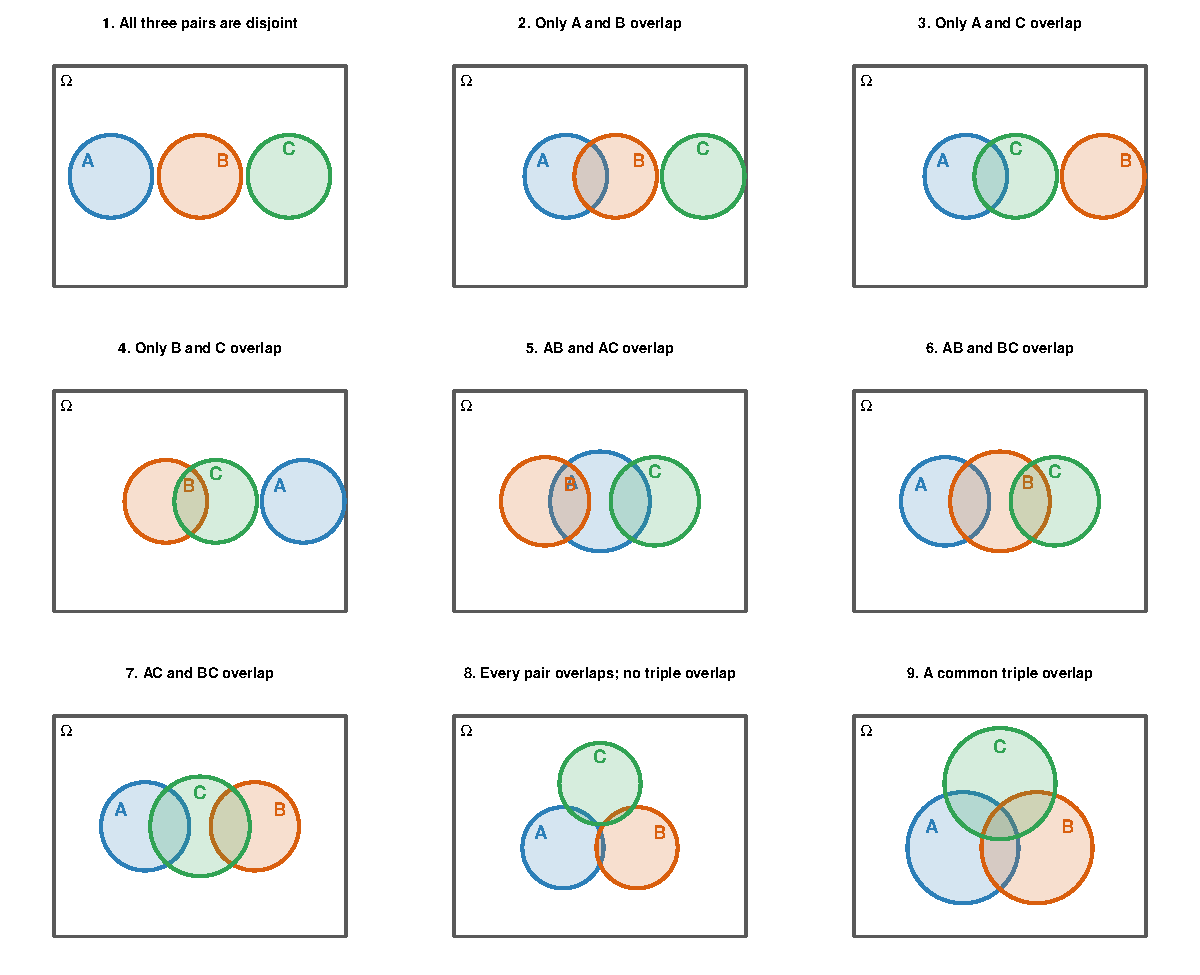
\includegraphics[width=0.85\textwidth]{img/venn-configurations.pdf}
  \caption{The nine configurations of disjointness and overlap for three events.}
\end{figure}

\subsubsection{Basic set identities}

\mprop{Set identities}{
  For events $A, B, C$:
  \begin{itemize}
    \item complement laws: $A \cup A^c = \Omega$, $A \cap A^c = \varnothing$;
    \item commutative laws: $A \cap B = B \cap A$, $A \cup B = B \cup A$;
    \item distributive laws: $A \cap (B \cup C) = (A \cap B) \cup (A \cap C)$, $A \cup (B \cap C) = (A \cup B) \cap (A \cup C)$;
    \item De Morgan's laws: $(A \cup B)^c = A^c \cap B^c$, $(A \cap B)^c = A^c \cup B^c$.
  \end{itemize}
}

\pf{Proof}{
  Each identity is proved by \emph{double inclusion}, i.e.\ by checking that an outcome $\omega$ belongs to the left side iff it
  belongs to the right side.
  \begin{itemize}
    \item Complement and commutative laws: $\omega \in A$ or $\omega \notin A$, never both; ``and'' and ``or'' are symmetric.
    \item Distributive: $\omega \in A \cap (B \cup C)$ $\iff$ $\omega \in A$ and ($\omega \in B$ or $\omega \in C$) $\iff$
          ($\omega \in A$ and $\omega \in B$) or ($\omega \in A$ and $\omega \in C$) $\iff$ $\omega \in (A \cap B) \cup (A \cap C)$.
          The second law is the same with ``and'' and ``or'' exchanged.
    \item De Morgan: $\omega \in (A \cup B)^c$ $\iff$ not ($\omega \in A$ or $\omega \in B$) $\iff$ $\omega \notin A$ and $\omega \notin B$
          $\iff$ $\omega \in A^c \cap B^c$. Applying this to $A^c, B^c$ and taking complements gives $(A \cap B)^c = A^c \cup B^c$.
  \end{itemize}
}

\textit{Suggested exercise 32.}

\subsection{Probability function}

\dfn{Probability function}{
  A \emph{probability function} is a mapping $\PP : \mathcal{A} \to [0,1]$, where $\mathcal{A}$ is a collection of events, such that
  \begin{itemize}
    \item $0 \leq \PP(A) \leq 1$ for all $A \in \mathcal{A}$;
    \item $\PP(\Omega) = 1$;
    \item $\PP(A \cup B) = \PP(A) + \PP(B) - \PP(A \cap B)$;
    \item for pairwise disjoint $A_1, A_2, \dots \in \mathcal{A}$: $\PP\big(\bigcup_{j \geq 1} A_j\big) = \sum_{j \geq 1} \PP(A_j)$.
  \end{itemize}
}

\mprop{Elementary consequences}{
  \begin{enumerate}
    \item $\PP(A^c) = 1 - \PP(A)$, in particular $\PP(\varnothing) = 0$;
    \item if $A \subseteq B$ then $\PP(A) \leq \PP(B)$;
    \item $\PP(A \cup B) \leq \PP(A) + \PP(B)$.
  \end{enumerate}
}

\pf{Proof}{
  \begin{enumerate}
    \item $A$ and $A^c$ are disjoint with $A \cup A^c = \Omega$, so $1 = \PP(\Omega) = \PP(A) + \PP(A^c)$. With $A = \Omega$: $\PP(\varnothing) = 0$.
    \item $B = A \cup (B \cap A^c)$ is a disjoint union, so $\PP(B) = \PP(A) + \PP(B \cap A^c) \geq \PP(A)$.
    \item From the union formula, since $\PP(A \cap B) \geq 0$.
  \end{enumerate}
  The union formula itself follows from additivity: $A \cup B = A \cup (B \cap A^c)$ and $B = (A \cap B) \cup (B \cap A^c)$ are disjoint
  unions, so $\PP(A \cup B) = \PP(A) + \PP(B) - \PP(A \cap B)$.
}

\subsubsection{Conditional probability}

\dfn{Conditional probability}{
  For events $A, B$ with $\PP(B) > 0$, the \emph{conditional probability} of $A$ given $B$ is
  \[
    \PP(A \mid B) = \frac{\PP(A \cap B)}{\PP(B)} .
  \]
  Conditioning restricts attention to the situations in which $B$ has occurred.
}

\teorema{
  \textbf{(Multiplication rule and Bayes' rule.)} If $\PP(B) > 0$, then $\PP(A \cap B) = \PP(A \mid B)\PP(B)$. If moreover $\PP(A) > 0$,
  \[
    \PP(A \mid B)\PP(B) = \PP(B \mid A)\PP(A)
    \qquad\text{and}\qquad
    \PP(A \mid B) = \frac{\PP(B \mid A)\PP(A)}{\PP(B)} .
  \]
}

\pf{Proof}{
  The multiplication rule is the definition multiplied by $\PP(B)$. Writing it both ways,
  $\PP(A \mid B)\PP(B) = \PP(A \cap B) = \PP(B \cap A) = \PP(B \mid A)\PP(A)$; dividing by $\PP(B)$ gives Bayes' rule.
}

\textit{Suggested exercise 33.}

\subsubsection{Law of total probability}

\teorema{
  \textbf{(Law of total probability.)} If $B_1, \dots, B_K$ form a \emph{partition} of $\Omega$ (pairwise disjoint,
  $\bigcup_k B_k = \Omega$) with $\PP(B_k) > 0$, then
  \[
    \PP(A) = \sum_{k=1}^{K} \PP(A \mid B_k)\PP(B_k) .
  \]
}

\pf{Proof}{
  By distributivity $A = A \cap \Omega = \bigcup_k (A \cap B_k)$, and the sets $A \cap B_k$ are pairwise disjoint (because the $B_k$ are).
  By additivity and the multiplication rule,
  $\PP(A) = \sum_k \PP(A \cap B_k) = \sum_k \PP(A \mid B_k)\PP(B_k)$.
}

\esempio{
  \textbf{Medical screening.} $D$ = ``has the condition'', $T$ = ``test positive'', with
  $\PP(D) = 0.02$, $\PP(T \mid D) = 0.95$ (sensitivity), $\PP(T \mid D^c) = 0.05$ (false positive rate).
  Total probability with the partition $\{D, D^c\}$:
  \[
    \PP(T) = 0.95 \cdot 0.02 + 0.05 \cdot 0.98 = 0.068 .
  \]
  Bayes' rule:
  \[
    \PP(D \mid T) = \frac{\PP(T \mid D)\PP(D)}{\PP(T)} = \frac{0.019}{0.068} \approx 0.279 .
  \]
  Even with an accurate test, a positive result means only a $28\%$ chance of having the condition: $\PP(T \mid D) = 0.95$ and
  $\PP(D \mid T) \approx 0.28$ are \red{different quantities}. The reason is the low prevalence: among $1000$ people, $\approx 19$ true
  positives against $\approx 49$ false positives.
}

\begin{lstlisting}
p_D <- 0.02; p_T_given_D <- 0.95; p_T_given_not_D <- 0.05
p_T <- p_T_given_D * p_D + p_T_given_not_D * (1 - p_D)   # 0.068
p_D_given_T <- p_T_given_D * p_D / p_T                    # 0.2794118
\end{lstlisting}

\subsubsection{Independence of events}

\dfn{Independence}{
  Events $A$ and $B$ are \emph{independent} if $\PP(A \cap B) = \PP(A)\PP(B)$.
}

\mprop{}{
  \begin{enumerate}
    \item If $\PP(B) > 0$: $A, B$ independent $\iff$ $\PP(A \mid B) = \PP(A)$ (learning $B$ does not change the probability of $A$).
    \item If $A, B$ are independent, so are $A$ and $B^c$.
    \item Two mutually exclusive events with positive probability are \red{never} independent.
  \end{enumerate}
}

\pf{Proof}{
  \begin{enumerate}
    \item $\PP(A \mid B) = \PP(A \cap B)/\PP(B)$ equals $\PP(A)$ iff $\PP(A \cap B) = \PP(A)\PP(B)$.
    \item $\PP(A \cap B^c) = \PP(A) - \PP(A \cap B) = \PP(A) - \PP(A)\PP(B) = \PP(A)(1 - \PP(B)) = \PP(A)\PP(B^c)$.
    \item $\PP(A \cap B) = \PP(\varnothing) = 0$, whereas $\PP(A)\PP(B) > 0$.
  \end{enumerate}
}

\textit{Suggested exercise 34.}

\subsection{Random variables}

\dfn{Random variable}{
  A \emph{random variable} is a function of the outcomes $X : \Omega \to \mathbb{S}_X$; the set $\mathbb{S}_X$ of possible values is the
  \emph{support}. For a set $B$ of values, the induced probability is
  \[
    \PP(X \in B) = \PP\big(\{\omega \in \Omega : X(\omega) \in B\}\big).
  \]
}

\esempio{
  Die roll: $X(\omega) = \omega$ (value of the die, $\mathbb{S}_X = \Omega$); $Y(\omega) = 1$ if $\omega$ is even and $0$ otherwise
  ($Y$ only records parity, $\mathbb{S}_Y = \{0, 1\}$). Then $\PP(Y = 1) = \PP(\{2,4,6\}) = 1/2$.
}

The support is usually \textbf{discrete finite} (e.g.\ $\{1, \dots, 6\}$), \textbf{discrete countably infinite} (e.g.\ $\{0, 1, 2, \dots\}$) or
\textbf{continuous} (e.g.\ $\mathbb{R}_+$).

\dfn{Cumulative distribution function}{
  The \emph{CDF} of $X$ is $F_X(x) = \PP(X \leq x)$, $x \in \mathbb{S}_X$. One writes $X \sim F_X$ (``is distributed according to''). It satisfies
  \begin{itemize}
    \item $0 \leq F_X(x) \leq 1$;
    \item $F_X$ is nondecreasing;
    \item $\lim_{x \to \inf \mathbb{S}_X} F_X(x) = 0$ and $\lim_{x \to \sup \mathbb{S}_X} F_X(x) = 1$.
  \end{itemize}
}

\osservazione{
  Monotonicity follows from the properties of $\PP$: if $x \leq y$ then $\{X \leq x\} \subseteq \{X \leq y\}$, so $F_X(x) \leq F_X(y)$.
  Moreover $\PP(a < X \leq b) = F_X(b) - F_X(a)$, since $\{X \leq b\}$ is the disjoint union of $\{X \leq a\}$ and $\{a < X \leq b\}$.
}

\dfn{Mass function and density}{
  \begin{itemize}
    \item \textbf{Discrete} $X$: probability mass function $\PP(X = x)$, and $F_X(x) = \sum_{t \leq x} \PP(X = t)$.
    \item \textbf{Continuous} $X$: a density $f_X \geq 0$ such that $\PP(a \leq X \leq b) = \int_a^b f_X(x)\,dx$, and
          $F_X(x) = \int_{\inf\mathbb{S}_X}^{x} f_X(t)\,dt$ (so $f_X = F_X'$ where differentiable).
  \end{itemize}
}

\mprop{Points have probability zero}{
  If $X$ is (absolutely) continuous, $\PP(X = a) = 0$ for every $a$, hence
  \[
    \PP(a < X < b) = \PP(a \leq X < b) = \PP(a < X \leq b) = \PP(a \leq X \leq b) .
  \]
}

\pf{Proof}{
  $\PP(X = a) = \int_a^a f_X(t)\,dt = 0$: a singleton has length zero. The four intervals differ only by the endpoints $\{a\}$ and $\{b\}$,
  which are disjoint from the rest and have probability $0$, so by additivity the probabilities coincide.
}

\textit{Suggested exercise 35.}

\subsection{Joint distributions}

\dfn{Joint density}{
  A pair $(X, Y)$ of continuous random variables is described by a joint density $f_{X,Y}(x,y) \geq 0$ with
  \[
    \int_{-\infty}^{\infty}\int_{-\infty}^{\infty} f_{X,Y}(x,y)\,dx\,dy = 1
  \]
  ($f_{X,Y} = 0$ outside the supports). Probabilities of regions are integrals, e.g.\
  $\PP(X \leq a, Y \leq b) = \int_{-\infty}^{a}\int_{-\infty}^{b} f_{X,Y}(x,y)\,dy\,dx$.
}

\dfn{Marginal and conditional densities}{
  \[
    f_X(x) = \int_{-\infty}^{\infty} f_{X,Y}(x,y)\,dy, \qquad
    f_Y(y) = \int_{-\infty}^{\infty} f_{X,Y}(x,y)\,dx, \qquad
    f_{Y \mid X}(y \mid x) = \frac{f_{X,Y}(x,y)}{f_X(x)} \ \ (f_X(x) > 0).
  \]
  In the discrete case integrals become sums.
}

\osservazione{
  The marginal is a density: $f_X \geq 0$ and $\int f_X(x)\,dx = \iint f_{X,Y} = 1$. Integrating out $y$ means ``ignoring $Y$'':
  $\PP(X \leq a) = \PP(X \leq a, Y \in \mathbb{R}) = \int_{-\infty}^{a}\big(\int f_{X,Y}(x,y)\,dy\big)dx$. Also the conditional density
  integrates to one in $y$: $\int f_{Y\mid X}(y \mid x)\,dy = f_X(x)/f_X(x) = 1$.
}

\dfn{Independent random variables}{
  $X$ and $Y$ are independent if $f_{X,Y}(x,y) = f_X(x)f_Y(y)$ for all $x, y$ (continuous case), or
  $\PP(X = x, Y = y) = \PP(X = x)\PP(Y = y)$ (discrete case). Equivalently $f_{Y\mid X}(y \mid x) = f_Y(y)$.
}

\textit{Suggested exercise 36.}

\subsection{Empirical distribution function}

A distribution $F_X$ can be interpreted as a \textbf{data generating process}: repeated draws of $X$ generate observations
distributed according to $F_X$.
\begin{itemize}
  \item A \textbf{random sample} $X_1, \dots, X_n$ consists of copies of the same random variable $X$, usually assumed
        \textbf{independent and identically distributed} (i.i.d.); it is used to study sample quantities (means, estimators).
  \item The \textbf{observed data} $x_1, \dots, x_n \in \mathbb{S}_X$ are realizations of them: the \emph{sample}.
\end{itemize}

\dfn{Empirical distribution function (EDF)}{
  \[
    F^{(n)}(x) = \frac{1}{n}\sum_{i=1}^{n} \mathbf{1}(x_i \leq x),
    \qquad
    \mathbf{1}(A) = \begin{cases} 1 & A \text{ true} \\ 0 & A \text{ false} \end{cases}
  \]
  It plays, for the observed sample, the role that $F_X$ plays for the population: it is the CDF of the distribution putting mass
  $1/n$ on each observation (a step function with jumps of $1/n$).
}

\mprop{The EDF estimates the CDF}{
  For an i.i.d.\ sample from $F_X$ and a fixed $x$, $nF^{(n)}(x) \sim \mathcal{B}(n, F_X(x))$, hence
  \[
    \EE\big[F^{(n)}(x)\big] = F_X(x), \qquad \Var\big(F^{(n)}(x)\big) = \frac{F_X(x)\big(1 - F_X(x)\big)}{n} \longrightarrow 0 .
  \]
}

\pf{Proof}{
  The indicators $\mathbf{1}(X_i \leq x)$ are i.i.d.\ Bernoulli with success probability $\PP(X_i \leq x) = F_X(x)$, so their sum is
  binomial (see the Bernoulli and binomial distributions below). Dividing the binomial mean $nF_X(x)$ and variance $nF_X(x)(1-F_X(x))$
  by $n$ and $n^2$ gives the claim.
}

\textit{Suggested exercise 37.}

\begin{lstlisting}
x  <- rnorm(100, mean = 0, sd = 1)
Fn <- ecdf(x)
plot(Fn, main = "Empirical distribution")
curve(pnorm(x), add = TRUE, lty = 2)
\end{lstlisting}

\begin{figure}[H]
  \centering
  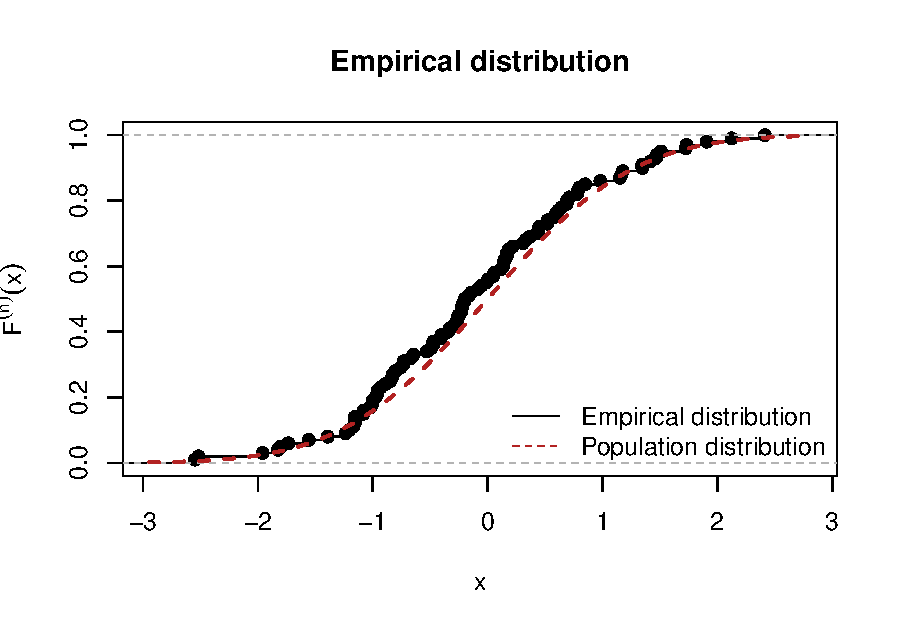
\includegraphics[width=0.6\textwidth]{img/edf.pdf}
  \caption{EDF of $100$ draws from $\mathcal{N}(0,1)$ (steps) and the population CDF $\Phi$ (dashed).}
\end{figure}

% ---------------------------------------------------------------------
\subsection{Moments}

A \emph{moment} summarizes an aspect of a distribution: the mean (location), the variance (spread), higher-order moments (shape).
\textbf{Population moments} are computed with $F_X$, \textbf{empirical moments} with $F^{(n)}$.

\dfn{Population moment}{
  For a suitable function $g$,
  \[
    \EE[g(X)] = \int_{\mathbb{S}_X} g(x)\,dF_X(x) = \int_{\mathbb{S}_X} g(x) f_X(x)\,dx ,
  \]
  since $dF_X(x) = f_X(x)\,dx$ in the continuous case.
}

\dfn{Expectation and variance}{
  \begin{itemize}
    \item \textbf{Expectation} (first moment, population mean, $g(x) = x$): $\mu = \EE[X] = \int x\,dF_X(x)$. It describes the
          centre of the distribution.
    \item \textbf{Second raw moment}: $\EE[X^2] = \int x^2\,dF_X(x)$.
    \item \textbf{Variance} (second \emph{central} moment):
          \[
            \sigma^2 = \Var(X) = \EE\big[(X - \mu)^2\big] = \int (x - \mu)^2\,dF_X(x) \geq 0 .
          \]
  \end{itemize}
}

\mprop{Variance from the first two raw moments}{
  \[
    \Var(X) = \EE[X^2] - \big(\EE[X]\big)^2 .
  \]
}

\pf{Proof}{
  Expand the square and use linearity of the integral, with $\mu$ a constant and $\int dF_X = 1$:
  \[
    \EE[(X - \mu)^2] = \EE[X^2] - 2\mu\EE[X] + \mu^2 = \EE[X^2] - 2\mu^2 + \mu^2 = \EE[X^2] - \mu^2 .
  \]
  In particular $\EE[X^2] \geq (\EE[X])^2$, since the variance is nonnegative.
}

\textit{Suggested exercises 38 and 39.}

\subsubsection{Discrete case}

If $X$ is discrete, $dF_X(x) = \PP(X = x)$ for $x \in \mathbb{S}_X$ and $0$ otherwise, so
\[
  \EE[g(X)] = \sum_{x \in \mathbb{S}_X} g(x)\PP(X = x) .
\]

\esempio{
  Fair die: $\EE[X] = \frac{1+\dots+6}{6} = 3.5$, $\EE[X^2] = \frac{1+4+9+16+25+36}{6} = \frac{91}{6}$, so
  $\Var(X) = \frac{91}{6} - \frac{49}{4} = \frac{35}{12} \approx 2.92$.
}

\subsubsection{Properties}

\mprop{Properties of expectation and variance}{
  For constants $a, b, c \in \mathbb{R}$:
  \begin{enumerate}
    \item $\EE[c] = c$; \quad $\EE[aX + bY] = a\EE[X] + b\EE[Y]$, and $\EE\big[\sum_i a_iX_i\big] = \sum_i a_i\EE[X_i]$; \quad $\EE[aX + b] = a\EE[X] + b$;
    \item if $X, Y$ are independent, $\EE[XY] = \EE[X]\EE[Y]$ (the converse is false in general);
    \item $\Var(c) = 0$, \quad $\Var(X + b) = \Var(X)$, \quad $\Var(aX) = a^2\Var(X)$, \quad $\Var(aX + b) = a^2\Var(X)$;
    \item $\Var(aX + bY) = a^2\Var(X) + b^2\Var(Y) + 2ab\Cov(X,Y)$, in particular $\Var(X + Y) = \Var(X) + \Var(Y) + 2\Cov(X,Y)$;
    \item if $X, Y$ are independent, $\Cov(X,Y) = 0$ and $\Var(X + Y) = \Var(X) + \Var(Y)$; more generally, for independent
          $X_1, \dots, X_n$, $\Var\big(\sum_i a_iX_i\big) = \sum_i a_i^2\Var(X_i)$.
  \end{enumerate}
}

\pf{Proof}{
  \begin{enumerate}
    \item Linearity of the integral (sum): $\EE[aX + bY] = \iint (ax + by) f_{X,Y}\,dx\,dy = a\int x f_X\,dx + b\int y f_Y\,dy$, using the
          marginals. $\EE[c] = c\int dF = c$. The finite-sum version follows by induction.
    \item By independence $f_{X,Y} = f_Xf_Y$, so $\EE[XY] = \iint xy\, f_X(x)f_Y(y)\,dx\,dy = \int x f_X(x)\,dx \int y f_Y(y)\,dy$.
    \item With $\mu = \EE[X]$: $\EE[aX + b] = a\mu + b$, hence
          $\Var(aX + b) = \EE\big[(aX + b - a\mu - b)^2\big] = a^2\EE[(X - \mu)^2] = a^2\Var(X)$. The other three are special cases
          ($a = 0$; $a = 1$; $b = 0$).
    \item With $\mu_X, \mu_Y$ the means,
          $\Var(aX + bY) = \EE\big[(a(X - \mu_X) + b(Y - \mu_Y))^2\big] = a^2\Var(X) + b^2\Var(Y) + 2ab\,\EE[(X - \mu_X)(Y - \mu_Y)]$.
    \item $\Cov(X,Y) = \EE[XY] - \EE[X]\EE[Y] = 0$ by point 2. For $n$ variables,
          $\Var\big(\sum_i a_iX_i\big) = \sum_i a_i^2\Var(X_i) + \sum_{i \neq j} a_ia_j\Cov(X_i, X_j)$ by the same expansion, and all
          covariances vanish.
  \end{enumerate}
}

\esempio{
  \textbf{Uncorrelated but dependent.} Let $X \sim \mathcal{N}(0,1)$ and $Y = X^2$. Then $\Cov(X, Y) = \EE[X^3] - \EE[X]\EE[X^2] = 0$
  (odd moments of a symmetric distribution vanish), but $Y$ is a function of $X$, so they are clearly not independent. This is why
  ``$\EE[XY] = \EE[X]\EE[Y]$'' does not imply independence.
}

\textit{Suggested exercise 40.}

\subsubsection{Covariance}

\dfn{Covariance}{
  For jointly distributed $X, Y$ with finite second moments,
  \[
    \Cov(X, Y) = \EE\big[(X - \EE[X])(Y - \EE[Y])\big] = \EE[XY] - \EE[X]\EE[Y] .
  \]
  Positive: large values of one tend to occur with large values of the other; negative: large with small; near zero: little
  \emph{linear} association (it does not imply independence).
}

\pf{Why the two expressions agree}{
  Expanding, $\EE[(X - \mu_X)(Y - \mu_Y)] = \EE[XY] - \mu_X\EE[Y] - \mu_Y\EE[X] + \mu_X\mu_Y = \EE[XY] - \mu_X\mu_Y$.
}

If $X, Y$ are independent (finite second moments) then $\Cov(X,Y) = 0$; the converse is generally false. The covariance enters the
variance of a sum: $\Var(X + Y) = \Var(X) + \Var(Y) + 2\Cov(X,Y)$.

\textit{Suggested exercise 41.}

\subsubsection{Correlation}

\dfn{Correlation}{
  \[
    \rho_{X,Y} = \Cor(X, Y) = \frac{\Cov(X,Y)}{\sqrt{\Var(X)\Var(Y)}} .
  \]
}

\teorema{
  \begin{enumerate}
    \item $-1 \leq \rho_{X,Y} \leq 1$, with $|\rho_{X,Y}| = 1$ iff $Y = aX + b$ almost surely for some $a \neq 0$;
    \item correlation is invariant to positive changes of scale: $\Cor(aX + c, bY + d) = \Cor(X, Y)$ for $ab > 0$ (and it changes
          sign if $ab < 0$).
  \end{enumerate}
}

\pf{Proof}{
  \textbf{1.} Let $U = (X - \mu_X)/\sigma_X$ and $V = (Y - \mu_Y)/\sigma_Y$, so $\EE[U^2] = \EE[V^2] = 1$ and $\EE[UV] = \rho$. Then
  \[
    0 \leq \EE\big[(U - V)^2\big] = 2 - 2\rho, \qquad 0 \leq \EE\big[(U + V)^2\big] = 2 + 2\rho,
  \]
  hence $-1 \leq \rho \leq 1$. Equality $\rho = 1$ means $\EE[(U - V)^2] = 0$, i.e.\ $U = V$ almost surely, a linear relation between
  $X$ and $Y$ with positive slope (similarly $\rho = -1$ with negative slope).

  \textbf{2.} Constants do not change covariances or variances, $\Cov(aX + c, bY + d) = ab\Cov(X,Y)$ and
  $\sqrt{\Var(aX + c)\Var(bY + d)} = |a||b|\sqrt{\Var(X)\Var(Y)}$, so $\Cor(aX + c, bY + d) = \frac{ab}{|ab|}\Cor(X,Y)$.
}

\textit{Suggested exercise 42.}

\subsubsection{Empirical moments}

For a sample $x_1, \dots, x_n$ the EDF puts mass $1/n$ on each observation ($dF^{(n)}(x_i) = 1/n$), so the plug-in moments are
\[
  \overline{x} = \int x\,dF^{(n)}(x) = \frac{1}{n}\sum_{i=1}^{n} x_i ,
  \qquad
  s^2 = \int (x - \overline{x})^2\,dF^{(n)}(x) = \frac{1}{n}\sum_{i=1}^{n} (x_i - \overline{x})^2
\]
(\emph{sample} or \emph{empirical} mean and variance), and for paired data $(x_i, y_i)$
\[
  \widehat{\Cov}(X, Y) = \frac{1}{n}\sum_{i=1}^{n} (x_i - \overline{x})(y_i - \overline{y}) .
\]

\osservazione{
  Empirical moments are close to, but not equal to, the population values: they depend on the random sample and fluctuate from
  sample to sample even when all samples come from the same $F_X$. The usual \emph{unbiased} sample covariance divides by $n - 1$;
  R's \texttt{cov()} and \texttt{var()} use this convention. The \textbf{correlation is unaffected} as long as the same denominator is
  used in the covariance and in the standard deviations (the factor cancels).
}

\mprop{Computational formulas}{
  \[
    \frac{1}{n}\sum_i (x_i - \overline{x})^2 = \frac{1}{n}\sum_i x_i^2 - \overline{x}^2,
    \qquad
    \frac{1}{n}\sum_i (x_i - \overline{x})(y_i - \overline{y}) = \frac{1}{n}\sum_i x_iy_i - \overline{x}\,\overline{y},
    \qquad
    \sum_i (x_i - \overline{x}) = 0 .
  \]
}

\pf{Proof}{
  These are $\Var(X) = \EE[X^2] - \EE[X]^2$ and $\Cov(X,Y) = \EE[XY] - \EE[X]\EE[Y]$ applied to the empirical distribution $F^{(n)}$.
  Directly: $\sum_i (x_i - \overline{x}) = n\overline{x} - n\overline{x} = 0$, and
  $\sum_i (x_i - \overline{x})(y_i - \overline{y}) = \sum_i x_iy_i - \overline{y}\sum_i x_i - \overline{x}\sum_i y_i + n\overline{x}\,\overline{y} = \sum_i x_iy_i - n\overline{x}\,\overline{y}$.
}

\textit{Suggested exercises 43 and 44.}

\begin{lstlisting}
set.seed(123)
n <- 200
x <- rnorm(n)
y <- 0.8 * x + rnorm(n, sd = 0.6)
c(covariance = cov(x, y), correlation = cor(x, y))
## covariance correlation
##  0.6960265  0.7772878
\end{lstlisting}

\esempio{
  Population values: $\Cov(X, Y) = \Cov(X, 0.8X + \varepsilon) = 0.8\Var(X) = 0.8$, $\Var(Y) = 0.64 + 0.36 = 1$, so
  $\rho = 0.8/\sqrt{1 \cdot 1} = 0.8$. The sample gives $0.696$ and $0.777$: close, but not equal.
}

\begin{figure}[H]
  \centering
  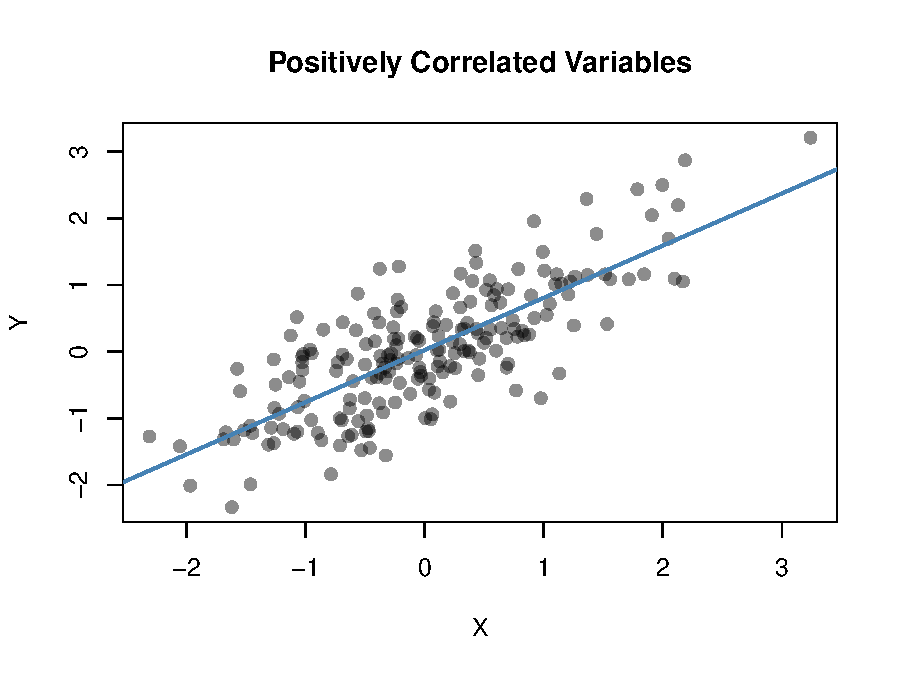
\includegraphics[width=0.55\textwidth]{img/correlated.pdf}
  \caption{Simulated positively correlated variables with the least-squares line.}
\end{figure}

% ---------------------------------------------------------------------
\subsection{Quantiles}

\dfn{Quantile}{
  For $p \in (0,1)$, a \emph{$p$-quantile} is a value $q_p$ with $F_X(q_p) \geq p$. The standard definition is the
  \emph{generalized inverse} of the CDF:
  \[
    q_p = \inf\{x \in \mathbb{S}_X : F_X(x) \geq p\} .
  \]
  If $F_X$ is continuous and strictly increasing, $q_p = F_X^{-1}(p)$, i.e.\ $F_X(q_p) = p$.
}

Special quantiles: the \textbf{median} $m = q_{0.5}$; the \textbf{quartiles} $q_{0.25}$, $q_{0.5}$, $q_{0.75}$; the
\textbf{$100p$-th percentile} is $q_p$ (e.g.\ the $90$-th percentile is $q_{0.90}$).

\textit{Suggested exercise 45.}

\begin{lstlisting}
qnorm(0.95)                    ## 1.644854
qbinom(0.95, size = 10, prob = 0.3)   ## 5
qunif(0.25, min = -1, max = 3) ## 0
qexp(0.5, rate = 2)            ## 0.3465736
set.seed(123); x <- rnorm(100)
quantile(x, probs = c(0.25, 0.5, 0.75))   # quantiles of the EDF
##         25%         50%         75%
## -0.49385424  0.06175631  0.69181917
\end{lstlisting}

\esempio{
  Checks by hand: $\mathcal{U}(-1, 3)$ has $F(x) = (x+1)/4$, so $q_{0.25}$ solves $(x+1)/4 = 0.25$, $x = 0$.
  $\operatorname{Exp}(2)$ has $F(x) = 1 - e^{-2x}$, so the median solves $e^{-2x} = 0.5$, $x = \log 2/2 \approx 0.3466$.
  For the discrete binomial the generalized inverse is needed: $5$ is the smallest $x$ with $F(x) \geq 0.95$.
}

% ---------------------------------------------------------------------
\subsection{Some well-known distributions}

\subsubsection{Bernoulli distribution}

\dfn{Bernoulli}{
  $X \sim \mathcal{B}(1, \pi)$ models a single binary outcome, $\mathbb{S}_X = \{0, 1\}$:
  $\PP(X = 1) = \pi$ (success), $\PP(X = 0) = 1 - \pi$ (failure); compactly
  \[
    \PP(X = x \mid \pi) = \pi^x(1 - \pi)^{1-x}, \qquad x \in \{0, 1\}.
  \]
  Examples: a coin flip, whether a customer clicks on an ad, whether a classifier's prediction is correct.
}

\mprop{Moments and quantiles of the Bernoulli}{
  $\EE[X] = \pi$, $\Var(X) = \pi(1 - \pi)$. The $p$-quantile is $0$ if $p \leq 1 - \pi$ and $1$ if $p > 1 - \pi$.
}

\pf{Proof}{
  $\EE[X] = 0 \cdot (1 - \pi) + 1 \cdot \pi = \pi$. Since $X^2 = X$ for $X \in \{0,1\}$, $\EE[X^2] = \pi$ and
  $\Var(X) = \pi - \pi^2 = \pi(1 - \pi)$. For the quantiles, $F_X(x) = 0$ for $x < 0$, $= 1 - \pi$ on $[0, 1)$, $= 1$ for $x \geq 1$:
  the smallest $x$ with $F_X(x) \geq p$ is $0$ when $p \leq 1 - \pi$, and $1$ otherwise.
}

So several probability levels correspond to the same quantile. In R: \texttt{rbinom(n, size = 1, prob = p)}.

\textit{Suggested exercise 46.}

\subsubsection{Binomial distribution}

\dfn{Binomial}{
  $X$ counts the successes in $N$ independent Bernoulli trials with success probability $\pi$: $\mathbb{S}_X = \{0, \dots, N\}$,
  $X \sim \mathcal{B}(N, \pi)$ and
  \[
    \PP(X = x \mid N, \pi) = \binom{N}{x}\pi^x(1 - \pi)^{N - x}, \qquad \binom{N}{x} = \frac{N!}{x!\,(N - x)!} .
  \]
}

\mprop{}{
  $\EE[X] = N\pi$, \quad $\Var(X) = N\pi(1 - \pi)$.
}

\pf{Proof}{
  \textbf{Mass function.} A specific sequence with $x$ successes and $N - x$ failures has probability $\pi^x(1 - \pi)^{N-x}$ by
  independence, and there are $\binom{N}{x}$ such sequences (choice of the positions of the successes).

  \textbf{Moments.} Write $X = \sum_{k=1}^{N} B_k$ with $B_k \iid \mathcal{B}(1, \pi)$. By linearity $\EE[X] = N\pi$; by independence
  $\Var(X) = \sum_k \Var(B_k) = N\pi(1 - \pi)$.
}

In R: \texttt{rbinom(n, size = N, prob = p)}.

\subsubsection{Uniform distribution}

\dfn{Uniform}{
  $X \sim \mathcal{U}(a, b)$ if all values of $[a, b]$ are equally plausible: $\mathbb{S}_X = [a, b]$,
  \[
    f_X(x) = \frac{1}{b - a} \ \ (a \leq x \leq b), \qquad F_X(x) = \frac{x - a}{b - a} \ \ (a \leq x \leq b).
  \]
}

\mprop{}{
  $\EE[X] = \dfrac{a + b}{2}$, \quad $\Var(X) = \dfrac{(b - a)^2}{12}$, \quad median $q_{0.5} = \dfrac{a + b}{2}$.
}

\pf{Proof}{
  \[
    \EE[X] = \int_a^b \frac{x}{b - a}\,dx = \frac{b^2 - a^2}{2(b - a)} = \frac{a + b}{2},
    \qquad
    \EE[X^2] = \int_a^b \frac{x^2}{b - a}\,dx = \frac{b^3 - a^3}{3(b - a)} = \frac{a^2 + ab + b^2}{3}.
  \]
  Hence $\Var(X) = \frac{a^2 + ab + b^2}{3} - \frac{(a + b)^2}{4} = \frac{4a^2 + 4ab + 4b^2 - 3a^2 - 6ab - 3b^2}{12} = \frac{(b - a)^2}{12}$.
  The median solves $\frac{x - a}{b - a} = \frac12$, i.e.\ $x = \frac{a + b}{2}$.
}

In R: \texttt{runif(10, min = -1, max = 1)}.

\textit{Suggested exercise 47.}

\teorema{
  \textbf{(Probability integral transform and inverse transform sampling.)} Let $X \sim F_X$ with $F_X$ continuous and strictly
  increasing. Then
  \[
    U = F_X(X) \sim \mathcal{U}(0, 1).
  \]
  Conversely, if $U \sim \mathcal{U}(0,1)$, then $X = F_X^{-1}(U)$ has CDF $F_X$.
}

\pf{Proof}{
  For $u \in [0,1]$, since $F_X$ is strictly increasing, $F_X(X) \leq u \iff X \leq F_X^{-1}(u)$, so
  \[
    \PP(U \leq u) = \PP(F_X(X) \leq u) = \PP\big(X \leq F_X^{-1}(u)\big) = F_X\big(F_X^{-1}(u)\big) = u ,
  \]
  which is the CDF of $\mathcal{U}(0,1)$. Conversely, $\PP(F_X^{-1}(U) \leq x) = \PP(U \leq F_X(x)) = F_X(x)$, because the uniform CDF
  is the identity on $[0,1]$.
}

\osservazione{
  This is why the uniform distribution is central in simulation: pseudo-random generators produce $\mathcal{U}(0,1)$ numbers, which are
  then transformed by $F_X^{-1}$. Example: for $\operatorname{Exp}(\lambda)$, $F^{-1}(u) = -\log(1 - u)/\lambda$, so
  $-\log(1 - U)/\lambda \sim \operatorname{Exp}(\lambda)$.
}

\textit{Suggested exercise 48.}

\subsubsection{Gaussian distribution}

\dfn{Gaussian (normal)}{
  $X \sim \mathcal{N}(\mu, \sigma^2)$ has density
  \[
    f(x \mid \mu, \sigma^2) = \frac{1}{\sqrt{2\pi\sigma^2}} \exp\Big( -\frac{(x - \mu)^2}{2\sigma^2} \Big),
    \qquad \EE[X] = \mu, \quad \Var(X) = \sigma^2 .
  \]
  It is the most important continuous distribution in statistics. Its CDF is denoted $\Phi$ when $\mu = 0$, $\sigma = 1$.
}

\teorema{
  \textbf{(Affine transformations.)} If $X \sim \mathcal{N}(\mu, \sigma^2)$ and $Y = aX + b$ with $a \neq 0$, then
  $Y \sim \mathcal{N}(a\mu + b, a^2\sigma^2)$. Consequently the \emph{standardized} variable
  \[
    Z = \frac{X - \mu}{\sigma} \sim \mathcal{N}(0, 1).
  \]
}

\pf{Proof}{
  Take $a > 0$ (the case $a < 0$ is analogous, with a sign flip). Then
  $F_Y(y) = \PP(aX + b \leq y) = F_X\big(\frac{y - b}{a}\big)$, and differentiating,
  \[
    f_Y(y) = \frac{1}{a} f_X\Big(\frac{y - b}{a}\Big)
    = \frac{1}{\sqrt{2\pi a^2\sigma^2}} \exp\Big( -\frac{\big(\frac{y - b}{a} - \mu\big)^2}{2\sigma^2} \Big)
    = \frac{1}{\sqrt{2\pi a^2\sigma^2}} \exp\Big( -\frac{(y - a\mu - b)^2}{2a^2\sigma^2} \Big),
  \]
  the $\mathcal{N}(a\mu + b, a^2\sigma^2)$ density. For $Z$ take $a = 1/\sigma$, $b = -\mu/\sigma$.
}

\textit{Suggested exercise 49.}

\subsubsection{Exponential distribution}

\dfn{Exponential}{
  $X \sim \operatorname{Exp}(\lambda)$, $\lambda > 0$, has density $f(x) = \lambda e^{-\lambda x}$ for $x \geq 0$. It is the standard model
  for a positive waiting time (inter-arrival times).
}

\mprop{}{
  $F(x) = 1 - e^{-\lambda x}$, \quad $\EE[X] = \dfrac{1}{\lambda}$, \quad $\Var(X) = \dfrac{1}{\lambda^2}$, \quad median $= \dfrac{\log 2}{\lambda}$.
}

\pf{Proof}{
  $F(x) = \int_0^x \lambda e^{-\lambda t}\,dt = 1 - e^{-\lambda x}$. By parts,
  \[
    \EE[X] = \int_0^\infty x\lambda e^{-\lambda x}dx = \big[-xe^{-\lambda x}\big]_0^\infty + \int_0^\infty e^{-\lambda x}dx = \frac{1}{\lambda},
    \qquad
    \EE[X^2] = \big[-x^2e^{-\lambda x}\big]_0^\infty + \int_0^\infty 2xe^{-\lambda x}dx = \frac{2}{\lambda}\EE[X] = \frac{2}{\lambda^2},
  \]
  so $\Var(X) = \frac{2}{\lambda^2} - \frac{1}{\lambda^2} = \frac{1}{\lambda^2}$. The median solves $e^{-\lambda x} = \frac12$.
}

In R: \texttt{rexp(10, rate = 2)}.

\subsubsection{Combinations of Gaussian random variables}

A sum of \emph{jointly Gaussian} random variables is Gaussian; its mean is the sum of the means, and its variance includes covariance
terms unless the variables are independent. In the independent case, if $X_j \sim \mathcal{N}(\mu_j, \sigma_j^2)$, $j = 1, \dots, p$,
\[
  \sum_{j=1}^{p} X_j \sim \mathcal{N}\Big( \sum_{j=1}^{p} \mu_j,\ \sum_{j=1}^{p} \sigma_j^2 \Big).
\]

\osservazione{
  The \emph{parameters} follow from the properties of moments alone (linearity of $\EE$, additivity of $\Var$ under independence);
  what is special to the Gaussian is that the \emph{shape} stays Gaussian. Combined with the affine property, the sample mean of
  i.i.d.\ $\mathcal{N}(\mu, \sigma^2)$ variables is exactly $\overline{X} \sim \mathcal{N}(\mu, \sigma^2/n)$.
  Generatively, a Gaussian produces observations concentrated around $\mu$ with spread governed by $\sigma^2$.
}

\begin{figure}[H]
  \centering
  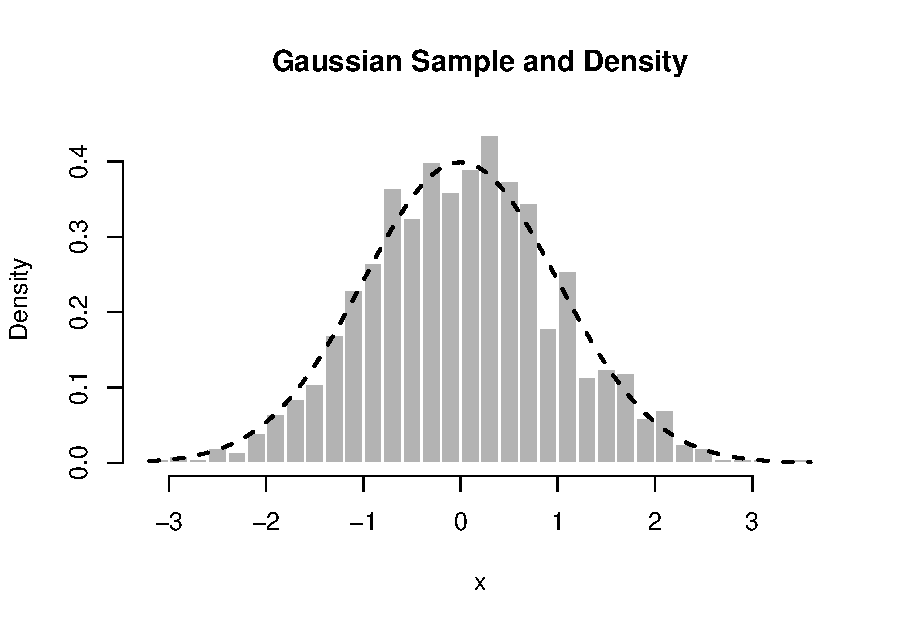
\includegraphics[width=0.55\textwidth]{img/gaussian-sample.pdf}
  \caption{Histogram of $1000$ draws from $\mathcal{N}(0,1)$ and the density.}
\end{figure}

\subsubsection{Multivariate Gaussian distribution}

\dfn{Multivariate Gaussian}{
  A random vector $\mathbf{X} \in \mathbb{R}^p$ is $\mathcal{N}(\boldsymbol{\mu}, \boldsymbol{\Sigma})$, with mean $\boldsymbol{\mu} \in \mathbb{R}^p$ and
  covariance matrix $\boldsymbol{\Sigma} \in \mathbb{R}^{p \times p}$ (symmetric positive definite), if its density is
  \[
    f(\mathbf{x} \mid \boldsymbol{\mu}, \boldsymbol{\Sigma}) = (2\pi)^{-p/2}|\boldsymbol{\Sigma}|^{-1/2}
    \exp\Big( -\frac12 (\mathbf{x} - \boldsymbol{\mu})^\top \boldsymbol{\Sigma}^{-1} (\mathbf{x} - \boldsymbol{\mu}) \Big).
  \]
}

\osservazione{
  \begin{itemize}
    \item For $p = 1$, $\boldsymbol{\Sigma} = \sigma^2$ and the formula reduces to the univariate density.
    \item If $\boldsymbol{\Sigma} = \operatorname{diag}(\sigma_1^2, \dots, \sigma_p^2)$, the quadratic form is $\sum_j (x_j - \mu_j)^2/\sigma_j^2$ and
          the density factorizes into the product of the marginals: uncorrelated jointly Gaussian components are \textbf{independent}
          (a property specific to the Gaussian).
    \item The population covariance matrix
          $\boldsymbol{\Sigma} = \EE\big[(\mathbf{X} - \EE[\mathbf{X}])(\mathbf{X} - \EE[\mathbf{X}])^\top\big]$ is exactly the object approximated by
          the empirical covariance matrix $\mathbf{S} = \frac1n\sum_i (\mathbf{x}_i - \overline{\mathbf{x}})(\mathbf{x}_i - \overline{\mathbf{x}})^\top$ of the PCA chapter:
          the multivariate Gaussian is the natural population model behind covariance matrices and PCA.
  \end{itemize}
}

\begin{lstlisting}
set.seed(123)
mu    <- c(0, 1)
Sigma <- matrix(c(1, 0.7,
                  0.7, 2), nrow = 2, byrow = TRUE)
X <- MASS::mvrnorm(n = 500, mu = mu, Sigma = Sigma)
\end{lstlisting}

\begin{figure}[H]
  \centering
  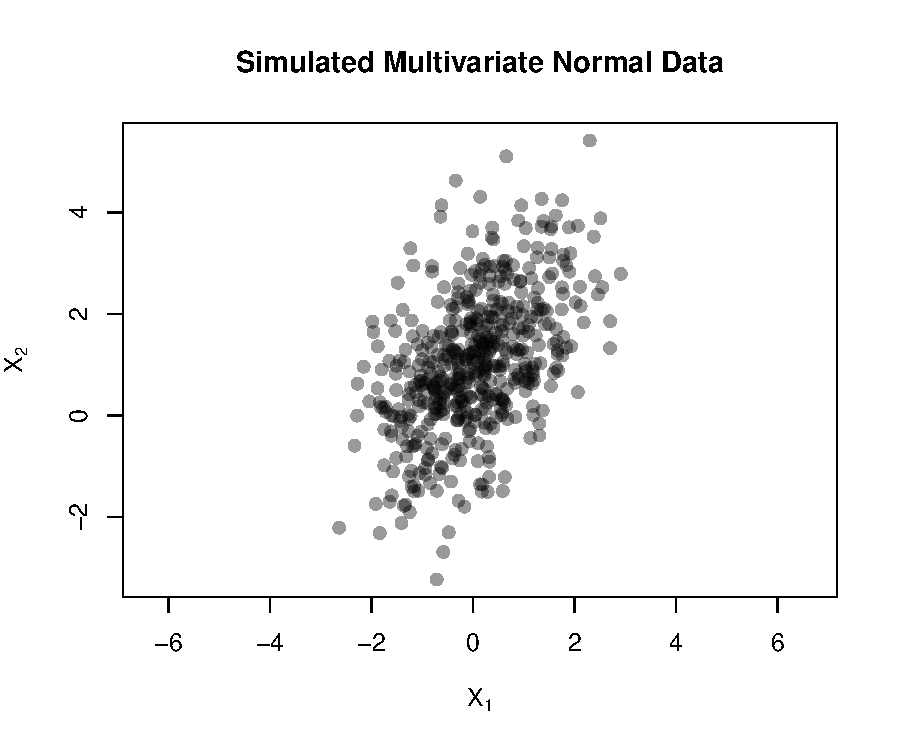
\includegraphics[width=0.5\textwidth]{img/mvnormal.pdf}
  \caption{$500$ draws from $\mathcal{N}(\boldsymbol{\mu}, \boldsymbol{\Sigma})$; the correlation is $0.7/\sqrt{2} \approx 0.49$.}
\end{figure}

% =====================================================================
\section{Estimation}

A distribution (\emph{statistical model}) structures our thinking about data; the observed data and their EDF contain information on
the underlying model. If a sample looks approximately normal, we may model it as $\mathcal{N}(\mu, \sigma^2)$ with \emph{unknown}
parameters. \textbf{Estimation} uses the data to learn the parameters of the data generating process.

\dfn{Point estimator}{
  A \emph{point estimator} is a function of the data $X_1, \dots, X_n$. Examples: the sample mean $\overline{x}$ for the population mean
  $\mu$; the empirical covariance matrix $\mathbf{S}$ for $\boldsymbol{\Sigma}$.
}

\subsection{Plug-in estimators}

\dfn{Plug-in estimator}{
  If the target is a \emph{functional} of the distribution, $\theta = T(F_X)$, the plug-in estimator replaces $F_X$ by the EDF:
  \[
    \widehat{\theta} = T\big(F^{(n)}\big).
  \]
}

\esempio{
  \[
    \mu = \int x\,dF_X(x) \ \Longrightarrow\ \widehat{\mu} = \int x\,dF^{(n)}(x) = \overline{x},
    \qquad
    \sigma^2 = \int (x - \mu)^2\,dF_X(x) \ \Longrightarrow\ \widehat{\sigma}^2 = \frac1n\sum_i (x_i - \overline{x})^2 .
  \]
  Likewise the median $q_{0.5}(F_X)$ is estimated by the sample median, and $\boldsymbol{\Sigma}$ by $\mathbf{S}$ (multivariate case).
}

\subsection{Maximum likelihood estimation}

\dfn{Likelihood and MLE}{
  Let the data be modelled by $\PP(X = x \mid \theta) = p(x \mid \theta)$ (a mass function or a density), with unknown parameter
  $\theta$. For i.i.d.\ observations $x_1, \dots, x_n$, the \emph{likelihood} is the joint probability of the sample as a function of $\theta$,
  \[
    L(\theta) = \prod_{i=1}^{n} p(x_i \mid \theta),
  \]
  and the \emph{maximum likelihood estimator} is $\widehat{\theta} = \arg\max_\theta L(\theta)$. One usually maximizes the
  \emph{log-likelihood}
  \[
    \ell(\theta) = \log L(\theta) = \sum_{i=1}^{n} \log p(x_i \mid \theta),
  \]
  which has the same maximizer because $\log$ is increasing, and turns products into sums.
}

\mprop{MLE of a Bernoulli}{
  If $X_1, \dots, X_n \iid \mathcal{B}(1, \pi)$, $\pi \in [0,1]$, then $\widehat{\pi} = \frac1n\sum_i x_i = \overline{x}$.
}

\pf{Proof}{
  With $p(x_i) = \pi^{x_i}(1 - \pi)^{1 - x_i}$ and $k = \sum_i x_i$ (number of successes),
  \[
    \ell(\pi) = \sum_{i=1}^{n} \big[x_i\log\pi + (1 - x_i)\log(1 - \pi)\big] = k\log\pi + (n - k)\log(1 - \pi).
  \]
  For $0 < k < n$:
  \[
    \ell'(\pi) = \frac{k}{\pi} - \frac{n - k}{1 - \pi} = 0 \iff k(1 - \pi) = (n - k)\pi \iff \pi = \frac{k}{n},
  \]
  and $\ell''(\pi) = -\frac{k}{\pi^2} - \frac{n-k}{(1-\pi)^2} < 0$, so it is a maximum. If $k = 0$ (resp.\ $k = n$), $\ell(\pi) = n\log(1 - \pi)$
  (resp.\ $n\log\pi$) is maximized at $\pi = 0$ (resp.\ $1$), again $k/n$.
}

So familiar empirical quantities are not only intuitive summaries: they also arise from a probabilistic estimation principle.

\textit{Suggested exercise 50.}

\mprop{MLE of a Gaussian}{
  If $X_1, \dots, X_n \iid \mathcal{N}(\mu, \sigma^2)$, then
  \[
    \widehat{\mu}_{\mathrm{ML}} = \overline{x}, \qquad \widehat{\sigma}^2_{\mathrm{ML}} = \frac1n\sum_{i=1}^{n} (x_i - \overline{x})^2 .
  \]
}

\pf{Proof}{
  \[
    \ell(\mu, \sigma^2) = \sum_{i=1}^{n} \log\Big[ \frac{1}{\sqrt{2\pi\sigma^2}} e^{-(x_i - \mu)^2/(2\sigma^2)} \Big]
    = -\frac{n}{2}\log(2\pi) - \frac{n}{2}\log\sigma^2 - \frac{1}{2\sigma^2}\sum_{i=1}^{n}(x_i - \mu)^2 .
  \]
  \textbf{In $\mu$}: for any $\sigma^2$, maximizing $\ell$ means minimizing $\sum_i (x_i - \mu)^2$;
  $\frac{\partial}{\partial\mu}\sum_i (x_i - \mu)^2 = -2\sum_i (x_i - \mu) = 0 \iff \mu = \overline{x}$ (a minimum, the function being a convex parabola).
  Equivalently, $\sum_i (x_i - \mu)^2 = \sum_i (x_i - \overline{x})^2 + n(\overline{x} - \mu)^2$.

  \textbf{In $\sigma^2$}: set $v = \sigma^2$ and $Q = \sum_i (x_i - \overline{x})^2$. Then
  $\frac{\partial\ell}{\partial v} = -\frac{n}{2v} + \frac{Q}{2v^2} = 0 \iff v = Q/n$; the derivative is positive for $v < Q/n$ and negative
  for $v > Q/n$, so this is the maximum.
}

\osservazione{
  For the Gaussian, the MLEs coincide with the plug-in estimators. Note that $\widehat{\sigma}^2_{\mathrm{ML}}$ divides by $n$: it is
  \emph{biased} (see below).
}

\textit{Suggested exercise 51.}

% ---------------------------------------------------------------------
\subsection{Properties of estimators}

\begin{itemize}
  \item An \textbf{estimator} is a function of the random sample $X_1, \dots, X_n$: it is itself a \emph{random variable}, with a
        \emph{sampling distribution} (often unknown, though some of its moments can be derived).
  \item An \textbf{estimate} is the value of the estimator on an observed sample.
\end{itemize}
The moments of the sampling distribution are used to study the properties of estimators.

\subsubsection{Bias}

\dfn{Bias}{
  $\operatorname{Bias}(\widehat{\theta}) = \EE[\widehat{\theta}] - \theta$. The estimator is \emph{unbiased} if $\EE[\widehat{\theta}] = \theta$:
  on average over repeated samples it hits the true parameter.
}

\mprop{The sample mean is unbiased}{
  If $X_1, \dots, X_n$ are i.i.d.\ with mean $\mu$, then $\EE[\overline{X}] = \mu$.
}

\pf{Proof}{
  By linearity, $\EE[\overline{X}] = \frac1n\sum_{i=1}^{n}\EE[X_i] = \frac1n \cdot n\mu = \mu$.
}

\subsubsection{Variance of an estimator}

\dfn{Variance and efficiency}{
  $\Var(\widehat{\theta}) = \EE\big[(\widehat{\theta} - \EE[\widehat{\theta}])^2\big]$; a good estimator has small variance. Among unbiased
  estimators of the same parameter, the one with smaller variance is more \emph{efficient}. The \emph{standard error} is
  $\sqrt{\Var(\widehat{\theta})}$.
}

\mprop{Variance of the sample mean}{
  If $X_1, \dots, X_n$ are i.i.d.\ with variance $\sigma^2$, then
  \[
    \Var(\overline{X}) = \frac{\sigma^2}{n}, \qquad \operatorname{se}(\overline{X}) = \frac{\sigma}{\sqrt{n}} .
  \]
}

\pf{Proof}{
  By independence, $\Var\big(\frac1n\sum_i X_i\big) = \frac{1}{n^2}\sum_i \Var(X_i) = \frac{1}{n^2} \cdot n\sigma^2 = \frac{\sigma^2}{n}$.
}

So increasing the sample size reduces the variability of the estimator. For Gaussian data,
$\overline{X}_n \sim \mathcal{N}(\mu, \sigma^2/n)$ exactly.

\begin{lstlisting}
set.seed(123)
B <- 5000; sample_sizes <- c(5, 10, 30, 100, 300); mu <- 2; sigma <- 3
# for each n: B sample means of Gaussian samples
xbar <- replicate(B, mean(rnorm(n, mean = mu, sd = sigma)))
\end{lstlisting}

\begin{center}
\begin{tabular}{cccccc}
  \hline
  $n$ & mean of $\overline{X}$ & bias & empirical var. & $\sigma^2/n$ & $\sigma/\sqrt{n}$ \\
  \hline
  5   & 1.9805 & $-0.0195$ & 1.8050 & 1.80 & 1.3416 \\
  10  & 2.0151 & $0.0151$  & 0.8786 & 0.90 & 0.9487 \\
  30  & 2.0156 & $0.0156$  & 0.3006 & 0.30 & 0.5477 \\
  100 & 1.9954 & $-0.0046$ & 0.0903 & 0.09 & 0.3000 \\
  300 & 1.9969 & $-0.0031$ & 0.0305 & 0.03 & 0.1732 \\
  \hline
\end{tabular}
\end{center}

\begin{figure}[H]
  \centering
  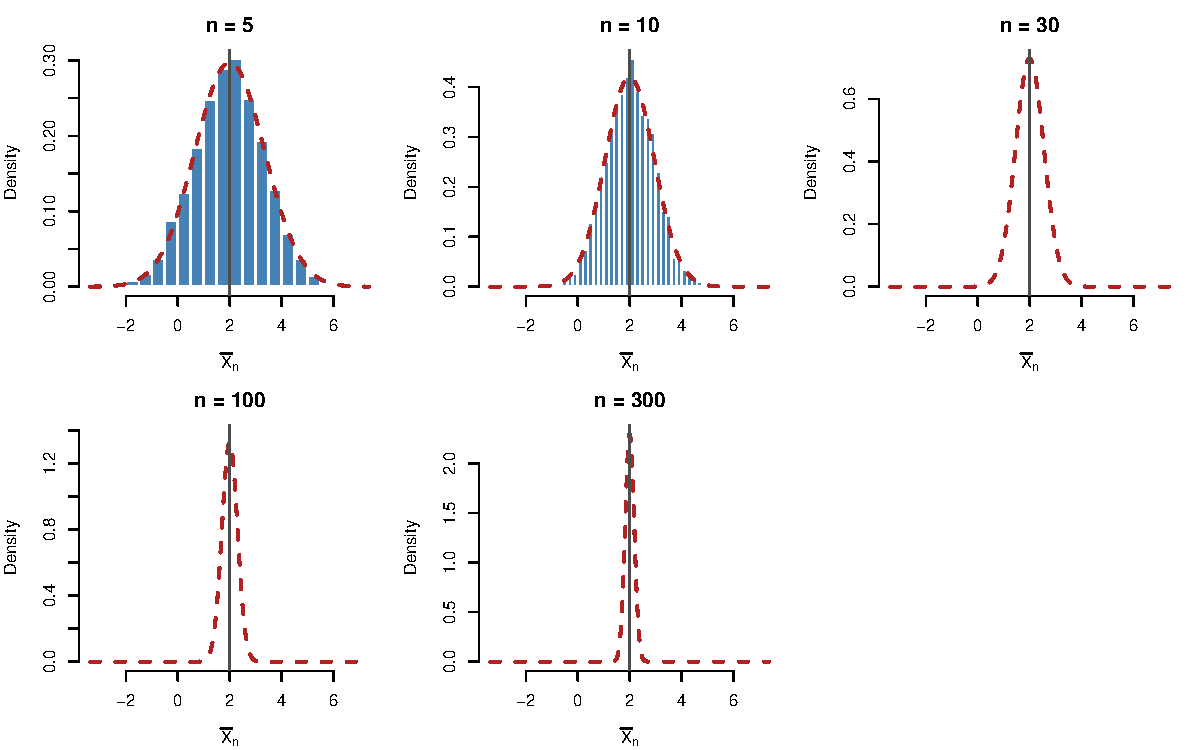
\includegraphics[width=0.9\textwidth]{img/xbar-sampling.pdf}
  \caption{Sampling distribution of $\overline{X}_n$ ($B = 5000$ replications) with the exact density $\mathcal{N}(\mu, \sigma^2/n)$ (dashed).}
\end{figure}

The simulation shows that the estimator is centred near $\mu$ (unbiasedness), has nonzero variance, and becomes more concentrated as
$n$ grows, in agreement with $\sigma^2/n$.

\subsubsection{Mean squared error}

\dfn{Mean squared error}{
  $\operatorname{MSE}(\widehat{\theta}) = \EE\big[(\widehat{\theta} - \theta)^2\big]$.
}

\teorema{
  \textbf{(Bias--variance decomposition.)}
  \[
    \operatorname{MSE}(\widehat{\theta}) = \Var(\widehat{\theta}) + \operatorname{Bias}(\widehat{\theta})^2 .
  \]
}

\pf{Proof}{
  Add and subtract $\EE[\widehat{\theta}]$:
  \[
    \EE\big[(\widehat{\theta} - \theta)^2\big]
    = \EE\big[(\widehat{\theta} - \EE[\widehat{\theta}])^2\big]
      + 2\big(\EE[\widehat{\theta}] - \theta\big)\underbrace{\EE\big[\widehat{\theta} - \EE[\widehat{\theta}]\big]}_{= 0}
      + \big(\EE[\widehat{\theta}] - \theta\big)^2 ,
  \]
  where $\EE[\widehat{\theta}] - \theta$ is a constant and can be taken out of the expectation.
}

This shows that an estimator with a small bias but a much smaller variance can be preferable to an unbiased one with high variance.

\textit{Suggested exercise 52.}

\mprop{Bias of the empirical variance}{
  If $X_1, \dots, X_n$ are i.i.d.\ with variance $\sigma^2$, then for $\widehat{\sigma}^2 = \frac1n\sum_i (X_i - \overline{X})^2$
  \[
    \EE\big[\widehat{\sigma}^2\big] = \frac{n - 1}{n}\sigma^2, \qquad \operatorname{Bias}(\widehat{\sigma}^2) = -\frac{\sigma^2}{n},
  \]
  while $s^2 = \frac{1}{n-1}\sum_i (X_i - \overline{X})^2$ is unbiased.
}

\pf{Proof}{
  By the computational formula, $\sum_i (X_i - \overline{X})^2 = \sum_i X_i^2 - n\overline{X}^2$. Using $\EE[Y^2] = \Var(Y) + \EE[Y]^2$,
  \[
    \EE[X_i^2] = \sigma^2 + \mu^2, \qquad \EE[\overline{X}^2] = \frac{\sigma^2}{n} + \mu^2 .
  \]
  Hence $\EE\big[\sum_i (X_i - \overline{X})^2\big] = n(\sigma^2 + \mu^2) - n\big(\frac{\sigma^2}{n} + \mu^2\big) = (n - 1)\sigma^2$. Dividing by $n$
  or by $n - 1$ gives the two statements. Intuitively, deviations are measured from $\overline{X}$, which is closer to the data than $\mu$:
  one ``degree of freedom'' is used to estimate the mean.
}

\subsubsection{Consistency}

Bias, variance and MSE are \emph{finite-sample} properties. When they cannot be computed explicitly, one studies the behaviour as
$n \to \infty$: \emph{asymptotic} properties.

\teorema{
  \textbf{(Weak law of large numbers.)} Let $X_1, X_2, \dots$ be i.i.d.\ from any $F_X$ with finite mean $\mu$. Then the sample mean
  converges in probability to $\mu$:
  \[
    \overline{X} \xrightarrow{\ \PP\ } \mu, \qquad\text{i.e.}\qquad \PP\big(|\overline{X} - \mu| > \varepsilon\big) \to 0 \quad \forall\varepsilon > 0 .
  \]
}

\pf{Proof (under the extra assumption of a finite variance $\sigma^2$)}{
  \textbf{Chebyshev's inequality}: for any $Y$ with finite variance and $\varepsilon > 0$,
  \[
    \PP\big(|Y - \EE[Y]| > \varepsilon\big) \leq \frac{\Var(Y)}{\varepsilon^2},
  \]
  because $\Var(Y) = \EE[(Y - \EE Y)^2] \geq \EE\big[(Y - \EE Y)^2\,\mathbf{1}(|Y - \EE Y| > \varepsilon)\big] \geq \varepsilon^2\,\PP(|Y - \EE Y| > \varepsilon)$.
  Applied to $Y = \overline{X}$, with $\EE[\overline{X}] = \mu$ and $\Var(\overline{X}) = \sigma^2/n$:
  \[
    \PP\big(|\overline{X} - \mu| > \varepsilon\big) \leq \frac{\sigma^2}{n\varepsilon^2} \longrightarrow 0 .
  \]
  (The general case with only a finite mean needs more advanced tools.)
}

\dfn{Consistency}{
  An estimator is \emph{consistent} if $\widehat{\theta} \xrightarrow{\PP} \theta$ as $n \to \infty$. The LLN says that $\overline{X}$ is
  consistent for $\mu$.
}

\osservazione{
  The same Chebyshev argument shows that \textbf{any estimator whose MSE tends to $0$ is consistent}:
  $\PP(|\widehat{\theta} - \theta| > \varepsilon) \leq \EE[(\widehat{\theta} - \theta)^2]/\varepsilon^2 = \operatorname{MSE}/\varepsilon^2$ (Markov's inequality
  applied to $(\widehat{\theta} - \theta)^2$). Hence a \emph{biased} estimator can be consistent, provided bias and variance both vanish:
  this is the case of $\widehat{\sigma}^2$ (bias $-\sigma^2/n$). Proving consistency in general requires fundamental theorems of
  statistics, ``left to statisticians''.
}

\subsubsection{Asymptotic normality}

\teorema{
  \textbf{(Central limit theorem.)} Let $X_1, \dots, X_n$ be i.i.d.\ from $F_X$ with mean $\mu$ and variance $\sigma^2 < \infty$, and
  $S_n = X_1 + \dots + X_n$, so that $\EE[S_n] = n\mu$ and $\Var(S_n) = n\sigma^2$. Then the standardized sum
  \[
    Z_n = \frac{S_n - n\mu}{\sqrt{n}\,\sigma} = \sqrt{n}\,\frac{\overline{X}_n - \mu}{\sigma}
  \]
  converges in distribution to $\mathcal{N}(0, 1)$. Informally, for moderately large $n$, $S_n \approx \mathcal{N}(n\mu, n\sigma^2)$ and
  $\overline{X}_n \approx \mathcal{N}(\mu, \sigma^2/n)$, \emph{whatever} the shape of $F_X$.
}

\osservazione{
  The moments of $S_n$ are exact and elementary (linearity and independence); the deep content of the CLT is that the \emph{shape}
  becomes Gaussian. The two expressions of $Z_n$ agree because $S_n - n\mu = n(\overline{X}_n - \mu)$ and $n/\sqrt{n} = \sqrt{n}$.
}

\esempio{
  \textbf{Sum of Gamma variables.} $X_i \iid \operatorname{Gamma}(\alpha, \theta)$ (shape $\alpha$, scale $\theta$) has
  $\EE[X_i] = \alpha\theta$, $\Var(X_i) = \alpha\theta^2$, so $\EE[S_n] = n\alpha\theta$, $\Var(S_n) = n\alpha\theta^2$. With $n = 30$,
  $\alpha = 2$, $\theta = 1.5$: $\EE[S_n] = 90$, $\operatorname{sd}(S_n) = \sqrt{30 \cdot 2 \cdot 2.25} = 11.619$. Although each $X_i$ is
  skewed, the histogram of $5000$ simulated sums is close to $\mathcal{N}(90, 11.619^2)$ (Monte Carlo mean $90.15$, sd $11.51$).
  Here $Z_n = \sqrt{n}\,(\overline{X}_n - \alpha\theta)/\sqrt{\alpha\theta^2}$.
}

\begin{lstlisting}
set.seed(123)
sum_gamma <- replicate(5000, sum(rgamma(30, shape = 2, scale = 1.5)))
\end{lstlisting}

\begin{figure}[H]
  \centering
  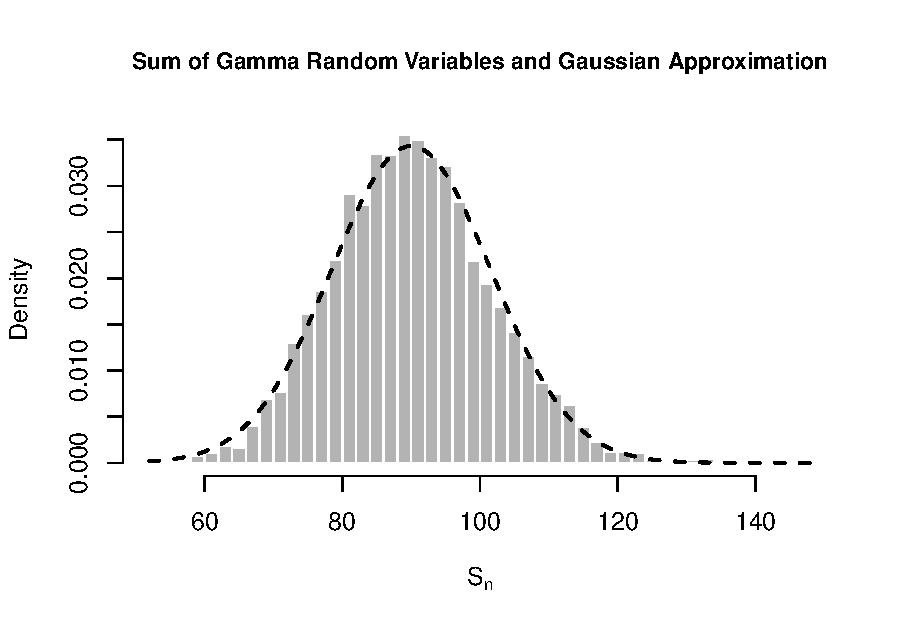
\includegraphics[width=0.6\textwidth]{img/clt-gamma.pdf}
  \caption{Simulated sums of $30$ Gamma variables and the Gaussian density with the same mean and variance.}
\end{figure}

\subsubsection{Monte Carlo study}

\dfn{Monte Carlo simulation}{
  Repeatedly generate data from a statistical model and compute quantities of interest:
  \begin{enumerate}
    \item choose a probability model and true parameter values;
    \item generate a sample from the model;
    \item compute a statistic or estimator;
    \item repeat many times ($B$ replications);
    \item study the distribution (EDF, histograms, boxplots) and moments of the outputs.
  \end{enumerate}
  It lets us study how estimators behave under controlled conditions, approximating their sampling distribution.
}

\esempio{
  \textbf{Bias and consistency of $\widehat{\sigma}^2$.} Gaussian samples with $\sigma^2 = 4$, $B = 5000$ replications for each $n$:

  \begin{center}
  \begin{tabular}{ccccc}
    \hline
    $n$ & MC mean of $\widehat{\sigma}^2$ & MC bias & MC sd & theory $\frac{n-1}{n}\cdot 4$ \\
    \hline
    3   & 2.6587 & $-1.3413$ & 2.6701 & 2.667 \\
    5   & 3.2063 & $-0.7937$ & 2.2687 & 3.200 \\
    10  & 3.6169 & $-0.3831$ & 1.7180 & 3.600 \\
    20  & 3.8204 & $-0.1796$ & 1.2352 & 3.800 \\
    50  & 3.9155 & $-0.0845$ & 0.7969 & 3.920 \\
    100 & 3.9560 & $-0.0440$ & 0.5419 & 3.960 \\
    500 & 3.9931 & $-0.0069$ & 0.2515 & 3.992 \\
    \hline
  \end{tabular}
  \end{center}

  The Monte Carlo means follow the theoretical value $\frac{n-1}{n}\sigma^2$ of the bias proposition: for $n = 3$ the estimator is
  clearly below $4$; as $n$ grows the bias and the spread vanish (consistency).
}

\begin{lstlisting}
s2_hat <- replicate(B, {
  x <- rnorm(n, mean = 0, sd = 2)
  mean((x - mean(x))^2)               # denominator n
})
\end{lstlisting}

\begin{figure}[H]
  \centering
  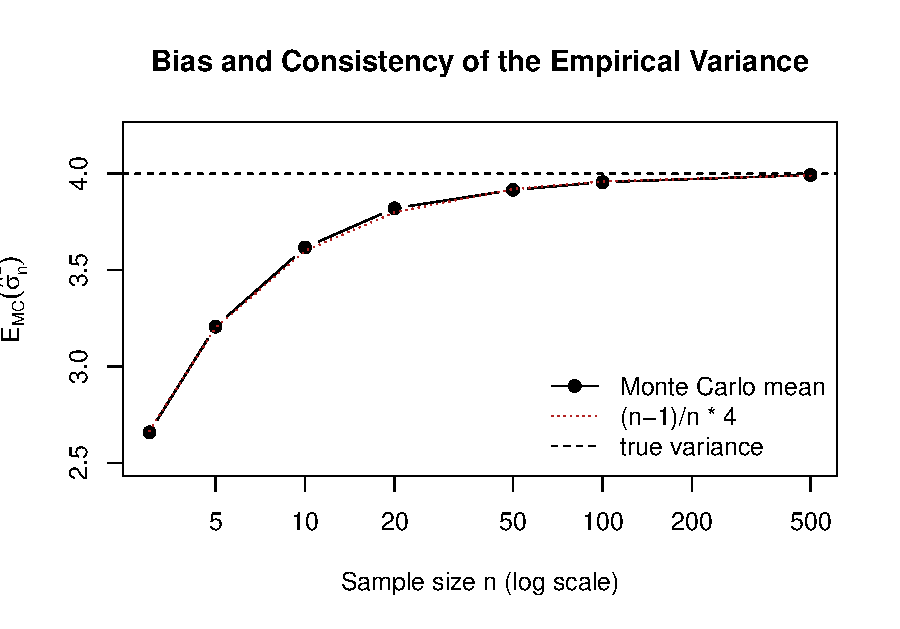
\includegraphics[width=0.55\textwidth]{img/variance-bias.pdf}
  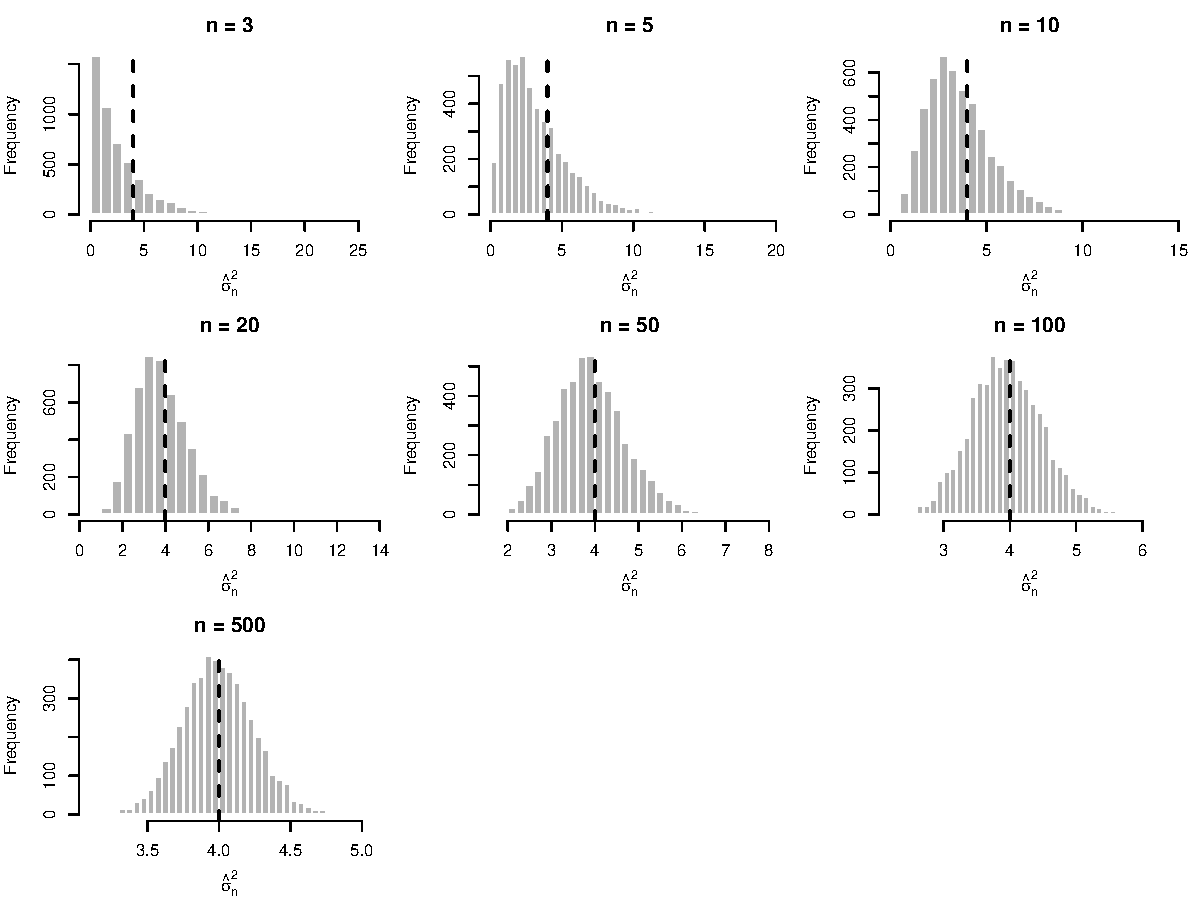
\includegraphics[width=0.85\textwidth]{img/variance-sampling.pdf}
  \caption{Top: Monte Carlo mean of $\widehat{\sigma}^2_n$ against $n$ (dashed: true value $4$). Bottom: sampling distributions; for small $n$
  they are very spread out and centred below the true value (dashed line).}
\end{figure}

% =====================================================================
\section{Interval Estimation}

Point estimators give one number but do not describe uncertainty; \textbf{confidence intervals} do.

\dfn{Confidence interval}{
  A confidence interval (CI) for $\theta$ is a \emph{random} interval $[C_l(X_1, \dots, X_n),\ C_u(X_1, \dots, X_n)]$ constructed so that,
  under repeated sampling, it contains the true $\theta$ with a prescribed probability $1 - \alpha$ (the \emph{confidence level},
  usually $95\%$). The bounds are functions of the random sample, hence random.
}

\subsection{Construction of confidence intervals}

A CI is built from the CDF $F_{\widehat{\theta}}$ of an unbiased or consistent estimator, derived theoretically or by simulation. It is
\textbf{exact} (valid for every $n$) or \textbf{asymptotic} (valid as $n \to \infty$; its accuracy at finite $n$ should then be checked,
e.g.\ by Monte Carlo). The recipe:
\begin{enumerate}
  \item find $T_l, T_u$ with $\PP(T_l \leq \widehat{\theta} \leq T_u) = \int_{T_l}^{T_u} dF_{\widehat{\theta}} = 1 - \alpha$ (a common choice is the
        central interval);
  \item since $F_{\widehat{\theta}}$ depends on $\theta$, \textbf{invert} the inequality into
        $\PP\big(g(T_l) \leq \theta \leq g(T_u)\big) = 1 - \alpha$, with bounds not depending on $\theta$;
  \item $[g(T_l), g(T_u)]$ is a $(1-\alpha)$ CI, exact or asymptotic according to $F_{\widehat{\theta}}$.
\end{enumerate}

\subsubsection{Example with an asymptotic CDF}

Asymptotically most consistent estimators are Gaussian: typically, via the CLT,
\[
  Z = \sqrt{n}\,\frac{\widehat{\theta} - \theta}{\sigma_{\widehat{\theta}}} \;\sim\; \mathcal{N}(0, 1) \quad\text{as } n \to \infty .
\]

\teorema{
  \textbf{(Asymptotic Gaussian CI.)} Let $z_{1-\alpha/2} = \Phi^{-1}(1 - \alpha/2)$. Then, asymptotically,
  \[
    \PP\Big( \widehat{\theta} - z_{1-\alpha/2}\frac{\sigma_{\widehat{\theta}}}{\sqrt{n}} \leq \theta \leq \widehat{\theta} + z_{1-\alpha/2}\frac{\sigma_{\widehat{\theta}}}{\sqrt{n}} \Big) = 1 - \alpha .
  \]
}

\pf{Proof}{
  Let $z_{\alpha/2} = \Phi^{-1}(\alpha/2)$. By symmetry of $\mathcal{N}(0,1)$, $z_{\alpha/2} = -z_{1-\alpha/2}$, and
  $\PP(z_{\alpha/2} < Z < z_{1-\alpha/2}) = (1 - \alpha/2) - \alpha/2 = 1 - \alpha$. Now invert:
  \[
    -z_{1-\alpha/2} < \sqrt{n}\,\frac{\widehat{\theta} - \theta}{\sigma_{\widehat{\theta}}} < z_{1-\alpha/2}
    \iff
    \widehat{\theta} - z_{1-\alpha/2}\frac{\sigma_{\widehat{\theta}}}{\sqrt{n}} < \theta < \widehat{\theta} + z_{1-\alpha/2}\frac{\sigma_{\widehat{\theta}}}{\sqrt{n}} ,
  \]
  multiplying by $\sigma_{\widehat{\theta}}/\sqrt{n} > 0$ and rearranging (the inequalities flip when isolating $-\theta$).
  For a continuous distribution strict and non-strict inequalities give the same probability.
}

\osservazione{
  The central interval is the \textbf{shortest} interval with probability $1-\alpha$ for the $\mathcal{N}(0,1)$, because the density is
  symmetric and unimodal. For $\alpha = 0.05$, $z_{0.975} = 1.96$. In practice the unknown $\sigma_{\widehat{\theta}}$ is replaced by a
  consistent estimate, e.g.\ for the mean $\overline{X} \pm 1.96\,s/\sqrt{n}$.
}

\textit{Suggested exercise 53.}

\begin{figure}[H]
  \centering
  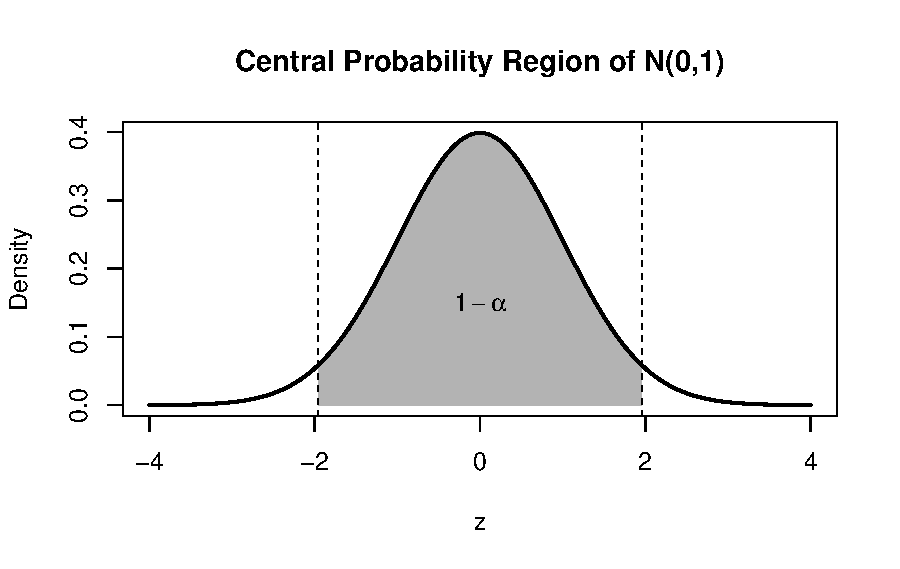
\includegraphics[width=0.55\textwidth]{img/ci-normal-region.pdf}
  \caption{The shaded region $z_{\alpha/2} < Z < z_{1-\alpha/2}$ has probability $1 - \alpha$.}
\end{figure}

\subsubsection{Example with an exact CDF}

\teorema{
  If $X_1, \dots, X_n \iid \mathcal{N}(\mu, \sigma^2)$ and $s^2 = \frac{1}{n-1}\sum_i (X_i - \overline{X})^2$, then
  \[
    \sqrt{n}\,\frac{\overline{X} - \mu}{s} \sim St_{n-1},
  \]
  the \emph{Student} distribution with $n - 1$ degrees of freedom (stated without proof). Hence the \textbf{exact} CI
  \[
    \mu \in \Big[ \overline{X} - t_{n-1,\,1-\alpha/2}\frac{s}{\sqrt{n}},\ \overline{X} + t_{n-1,\,1-\alpha/2}\frac{s}{\sqrt{n}} \Big].
  \]
}

\pf{Derivation of the interval}{
  The Student distribution is symmetric around $0$, so $\PP\big(-t_{n-1,1-\alpha/2} \leq T \leq t_{n-1,1-\alpha/2}\big) = 1 - \alpha$ for
  $T = \sqrt{n}(\overline{X} - \mu)/s$, and the inequalities are inverted exactly as in the Gaussian case.
}

\osservazione{
  The Student distribution has heavier tails than the Gaussian, so $t_{n-1,1-\alpha/2} > z_{1-\alpha/2}$ (e.g.\ $t_{9,0.975} = 2.262$ against
  $1.96$): the interval is wider to account for the estimation of $\sigma$ by $s$. As $n \to \infty$, $St_{n-1} \to \mathcal{N}(0,1)$ and the two
  intervals coincide. In R: \texttt{qt(0.975, df = n - 1)}.
}

\textit{Suggested exercise 54.}

\subsection{Bootstrap confidence intervals}

When the distribution of an estimator is hard to derive (even asymptotically), or its standard error is cumbersome, the
\textbf{bootstrap} gives a computational alternative.

\dfn{Nonparametric bootstrap}{
  Given the sample $x_1, \dots, x_n$ and a consistent estimator $\widehat{\theta}$:
  \begin{enumerate}
    \item resample $n$ observations \textbf{with replacement} from the data, $B$ times;
    \item compute the estimator on each resample: $\widehat{\theta}^{*1}, \dots, \widehat{\theta}^{*B}$ (bootstrap replicates);
    \item use the EDF of the replicates to approximate the sampling distribution of $\widehat{\theta}$.
  \end{enumerate}
  The \emph{percentile} interval is $[q^*_{\alpha/2},\ q^*_{1-\alpha/2}]$, with $q^*$ the empirical quantiles of the replicates.
}

\osservazione{
  Resampling from the data means sampling from the EDF $F^{(n)}$: the bootstrap is the plug-in principle applied to the
  \emph{whole} sampling distribution, i.e.\ ``the unknown $F_X$ is replaced by $F^{(n)}$''.
}

\esempio{
  \textbf{Median of an exponential sample.} The sample median has a much less convenient sampling distribution than the mean.
  We draw $n = 50$ observations from $\operatorname{Exp}(2)$, whose population median is $\log 2/2 \approx 0.3466$, and take $B = 10\,000$
  bootstrap samples.
  \begin{itemize}
    \item observed sample median $\widehat{\theta} = 0.4223$;
    \item bootstrap replicates: mean $0.4273$, variance $0.00635$, standard error $0.0797$;
    \item $95\%$ percentile CI: $[q^*_{0.025}, q^*_{0.975}] = [0.2919,\ 0.5896]$; with \texttt{boot::boot.ci} (different resamples):
          $[0.2919,\ 0.5960]$.
  \end{itemize}
  The two intervals differ only by Monte Carlo variation, which decreases with $B$. Here the interval contains the true median $0.3466$.
}

\begin{lstlisting}
set.seed(123)
x <- rexp(50, rate = 2)
theta_hat <- median(x)
set.seed(456)
theta_boot <- replicate(10000, median(sample(x, size = 50, replace = TRUE)))
quantile(theta_boot, probs = c(0.025, 0.975))     # percentile CI

# with the recommended package boot: statistic(data, indices)
median_statistic <- function(data, indices) median(data[indices])
boot_fit <- boot::boot(data = x, statistic = median_statistic, R = 10000)
boot::boot.ci(boot_fit, conf = 0.95, type = "perc")   # endpoints in $percent[4:5]
\end{lstlisting}

\begin{figure}[H]
  \centering
  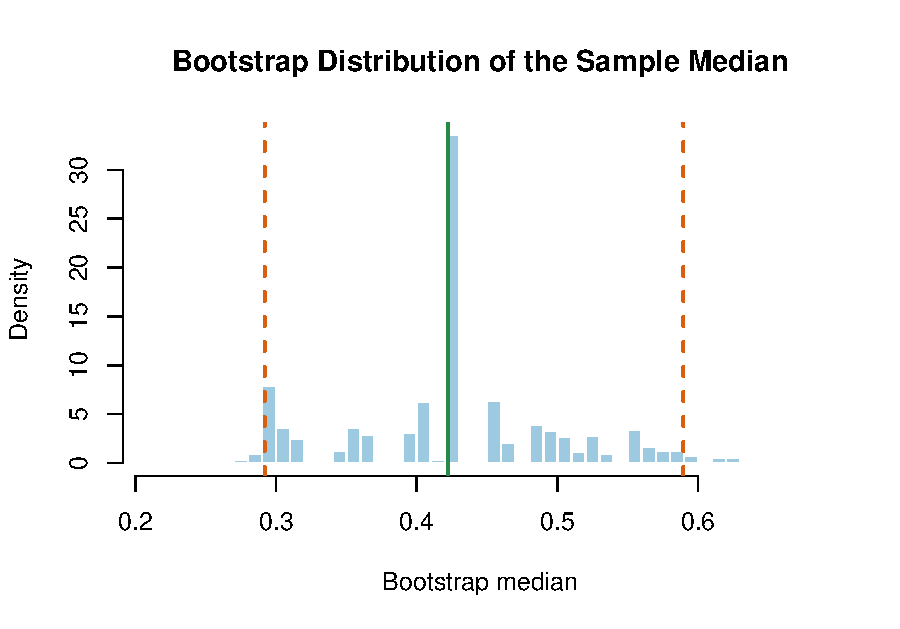
\includegraphics[width=0.6\textwidth]{img/bootstrap-median.pdf}
  \caption{Bootstrap distribution of the sample median: percentile endpoints (orange, dashed) and observed median (green).}
\end{figure}

\subsection{Coverage}

\dfn{Coverage probability}{
  For an interval procedure $[C_l(X_1, \dots, X_n), C_u(X_1, \dots, X_n)]$, the \emph{coverage} is
  \[
    \PP\big( C_l(X_1, \dots, X_n) \leq \theta \leq C_u(X_1, \dots, X_n) \big).
  \]
  A method advertised as a $95\%$ CI should have coverage close to $0.95$. Coverage is a property of the \textbf{procedure}, not of
  one realized interval: over many repetitions, about $95\%$ of the intervals should contain $\theta$.
}

\osservazione{
  Once the data are observed, a given interval either contains $\theta$ or not: the ``$95\%$'' refers to the random interval
  \emph{before} sampling.
}

\textbf{Monte Carlo estimate of coverage}: choose a model with known $\theta$ and a sample size $n$; generate many samples; compute the CI
on each; record whether it contains $\theta$; average. With $B$ replications, the estimate is the proportion of covering intervals
(a Bernoulli mean, with Monte Carlo standard error $\sqrt{0.95 \cdot 0.05/B} \approx 0.005$ for $B = 2000$).

\esempio{
  $X_1, \dots, X_n \iid \operatorname{Exp}(1)$ (skewed), $\theta = \EE[X] = 1$. Three $95\%$ CIs for the mean:
  \begin{itemize}
    \item \textbf{asymptotic Gaussian}: $\overline{X} \pm z_{0.975}\,s/\sqrt{n}$;
    \item \textbf{bootstrap normal}: $\overline{X} \pm z_{0.975}\,\widehat{\operatorname{se}}$, with $\widehat{\operatorname{se}}$ the standard deviation of the bootstrap means
          $\overline{X}^*_1, \dots, \overline{X}^*_B$;
    \item \textbf{bootstrap percentile}: empirical quantiles of the bootstrap means.
  \end{itemize}
  $B_{\mathrm{mc}} = 2000$ Monte Carlo samples, $B_{\mathrm{boot}} = 1000$ bootstrap replicates each. For $n = 30$:

  \begin{center}
  \begin{tabular}{lcc}
    \hline
    Method & Coverage & Average length \\
    \hline
    Asymptotic normal    & 0.9060 & 0.6959 \\
    Bootstrap normal     & 0.9020 & 0.6840 \\
    Bootstrap percentile & 0.9075 & 0.6781 \\
    \hline
  \end{tabular}
  \end{center}

  As a function of $n$:
  \begin{center}
  \begin{tabular}{lccccc}
    \hline
    $n$ & 10 & 20 & 30 & 50 & 100 \\
    \hline
    Asymptotic normal    & 0.8665 & 0.8975 & 0.9210 & 0.9450 & 0.9395 \\
    Bootstrap normal     & 0.8535 & 0.8885 & 0.9180 & 0.9435 & 0.9380 \\
    Bootstrap percentile & 0.8620 & 0.8930 & 0.9190 & 0.9410 & 0.9375 \\
    \hline
  \end{tabular}
  \end{center}

  A good method has coverage close to the nominal $0.95$ and intervals not unnecessarily wide. For small $n$ all three
  \textbf{undercover} (around $0.86$ at $n = 10$), because the skewness of the exponential makes the Gaussian approximation poor; the
  coverage approaches $0.95$ as $n$ grows. The two runs at $n = 30$ (0.906 vs 0.921) differ by Monte Carlo variation.
}

\begin{figure}[H]
  \centering
  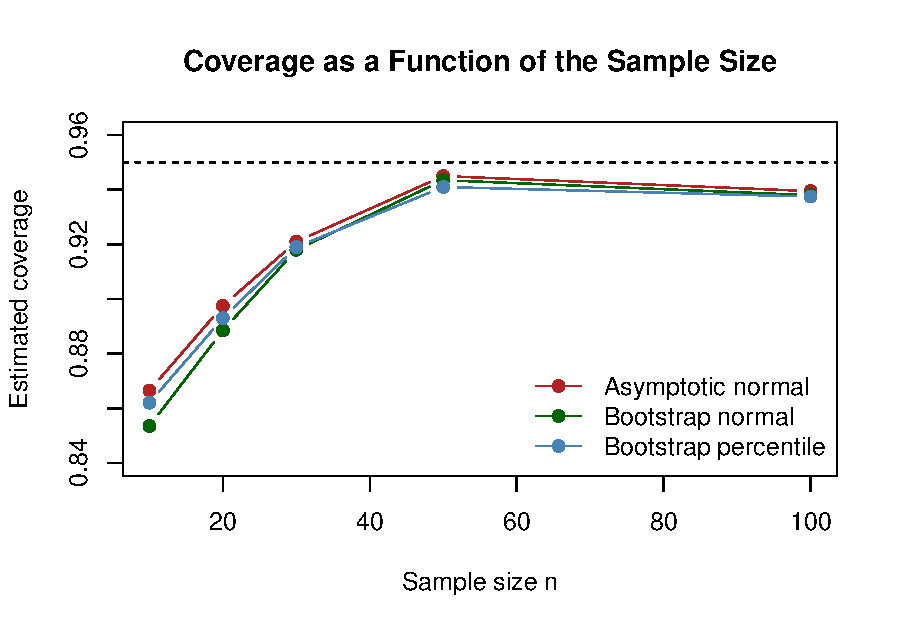
\includegraphics[width=0.6\textwidth]{img/coverage.pdf}
  \caption{Estimated coverage of the three $95\%$ CIs against $n$ (dashed: nominal level).}
\end{figure}
